\documentclass{beamer}
\usetheme[pageofpages=of,% String used between the current page and the
                         % total page count.
          bullet=circle,% Use circles instead of squares for bullets.
          titleline=true,% Show a line below the frame title.
          alternativetitlepage=true,% Use the fancy title page.
	  titlepagelogo=logo-circl.pdf,% Logo for the first page.
%          watermark=watermark-polito,% Watermark used in every page.
%          watermarkheight=100px,% Height of the watermark.
%          watermarkheightmult=4,% The watermark image is 4 times bigger
                                % than watermarkheight.
          ]{Torino}

\usepackage[utf8x]{inputenc}
\usepackage{listings}
\usepackage{soul}
\usepackage{siunitx}
\usepackage{booktabs}
%\lstset{ 
%  backgroundcolor=\color{white},   % choose the background color; you must add \usepackage{color} or \usepackage{xcolor}
%  basicstyle=\footnotesize,        % the size of the fonts that are used for the code
%  breakatwhitespace=false
%}

\usepackage{tikz}
\usetikzlibrary{shapes,snakes,automata,positioning,matrix,fit}


\usepackage[listings]{tcolorbox}
\usepackage{xcolor}
\usepackage{colortbl}
\definecolor{mygreen}{rgb}{0,0.6,0}
\definecolor{mygreen2}{rgb}{0,0.56,0.16}
\definecolor{myred}{rgb}{0.6,0.066,0.066}
\definecolor{redCIRCL}{RGB}{213,43,30}
\definecolor{mygray}{rgb}{0.5,0.5,0.5}
\definecolor{mymauve}{rgb}{0.58,0,0.82}
\definecolor{mygray}{gray}{0.9}
\definecolor{mywhite}{rgb}{1,1,1}
\definecolor{myblack}{rgb}{0,0,0}
\definecolor{mybeige}{HTML}{eeeeee}
%\usepackage{tcolorbox}
\usepackage[listings]{tcolorbox}
\tcbuselibrary{listings}

\lstdefinestyle{code}{ %
  backgroundcolor=\color{mybeige},   % choose the background color; you must add \usepackage{color} or \usepackage{xcolor}; should come as last argument
  basicstyle=\footnotesize\ttfamily,        % the size of the fonts that are used for the code
  breakatwhitespace=false,         % sets if automatic breaks should only happen at whitespace
  breaklines=true,                 % sets automatic line breaking
  captionpos=b,                    % sets the caption-position to bottom
  commentstyle=\color{mygreen},    % comment style
  deletekeywords={...},            % if you want to delete keywords from the given language
  escapeinside={\%*}{*)},          % if you want to add LaTeX within your code
  extendedchars=true,              % lets you use non-ASCII characters; for 8-bits encodings only, does not work with UTF-8
  frame=single,	                   % adds a frame around the code
  keepspaces=true,                 % keeps spaces in text, useful for keeping indentation of code (possibly needs columns=flexible)
  keywordstyle=\color{blue},       % keyword style
  language=Python,                 % the language of the code
  morekeywords={*,...},           % if you want to add more keywords to the set
  numbers=left,                    % where to put the line-numbers; possible values are (none, left, right)
  numbersep=5pt,                   % how far the line-numbers are from the code
  numberstyle=\tiny\color{myblack}, % the style that is used for the line-numbers
  rulecolor=\color{black},         % if not set, the frame-color may be changed on line-breaks within not-black text (e.g. comments (green here))
  showspaces=false,                % show spaces everywhere adding particular underscores; it overrides 'showstringspaces'
  showstringspaces=false,          % underline spaces within strings only
  showtabs=false,                  % show tabs within strings adding particular underscores
  stepnumber=1,                    % the step between two line-numbers. If it's 1, each line will be numbered
  stringstyle=\color{mymauve},     % string literal style
  tabsize=2,	                   % sets default tabsize to 2 spaces
  title=\lstname                   % show the filename of files included with \lstinputlisting; also try caption instead of title
}
\lstdefinestyle{bash}{ %
  backgroundcolor=\color{black!85},   % choose the background color; you must add \usepackage{color} or \usepackage{xcolor}; should come as last argument
  basicstyle=\footnotesize\color{mywhite},        % the size of the fonts that are used for the code
  breakatwhitespace=false,         % sets if automatic breaks should only happen at whitespace
  breaklines=true,                 % sets automatic line breaking
  captionpos=b,                    % sets the caption-position to bottom
  commentstyle=\color{mygreen},    % comment style
  deletekeywords={...},            % if you want to delete keywords from the given language
  escapeinside={\%*}{*)},          % if you want to add LaTeX within your code
  extendedchars=true,              % lets you use non-ASCII characters; for 8-bits encodings only, does not work with UTF-8
  frame=single	                   % adds a frame around the code
  keepspaces=true,                 % keeps spaces in text, useful for keeping indentation of code (possibly needs columns=flexible)
  keywordstyle=\color{white}\bfseries,       % keyword style
  language=bash,                 % the language of the code
  morekeywords={*,$,git, clone,... },           % if you want to add more keywords to the set
  numbers=left,                    % where to put the line-numbers; possible values are (none, left, right)
  numbersep=5pt,                   % how far the line-numbers are from the code
  numberstyle=\tiny\color{mywhite}, % the style that is used for the line-numbers
  rulecolor=\color{black},         % if not set, the frame-color may be changed on line-breaks within not-black text (e.g. comments (green here))
  showspaces=false,                % show spaces everywhere adding particular underscores; it overrides 'showstringspaces'
  showstringspaces=false,          % underline spaces within strings only
  showtabs=false,                  % show tabs within strings adding particular underscores
  stepnumber=1,                    % the step between two line-numbers. If it's 1, each line will be numbered
  stringstyle=\color{mymauve},     % string literal style
  tabsize=2,	                   % sets default tabsize to 2 spaces
  title=\lstname                   % show the filename of files included with \lstinputlisting; also try caption instead of title
}
\lstdefinestyle{default}{ %
  backgroundcolor=\color{white},   % choose the background color; you must add \usepackage{color} or \usepackage{xcolor}; should come as last argument
  basicstyle=\footnotesize\color{black},        % the size of the fonts that are used for the code
  breakatwhitespace=false,         % sets if automatic breaks should only happen at whitespace
  breaklines=true,                 % sets automatic line breaking
  captionpos=b,                    % sets the caption-position to bottom
  commentstyle=\color{mygreen},    % comment style
  deletekeywords={...},            % if you want to delete keywords from the given language
  escapeinside={\%*}{*)},          % if you want to add LaTeX within your code
  extendedchars=true,              % lets you use non-ASCII characters; for 8-bits encodings only, does not work with UTF-8
  frame=single	                   % adds a frame around the code
  keepspaces=true,                 % keeps spaces in text, useful for keeping indentation of code (possibly needs columns=flexible)
  keywordstyle=\color{white}\bfseries,       % keyword style
  language=bash,                 % the language of the code
  morekeywords={*,$,git, clone,... },           % if you want to add more keywords to the set
  numbers=left,                    % where to put the line-numbers; possible values are (none, left, right)
  numbersep=5pt,                   % how far the line-numbers are from the code
  numberstyle=\tiny\color{black}, % the style that is used for the line-numbers
  rulecolor=\color{black},         % if not set, the frame-color may be changed on line-breaks within not-black text (e.g. comments (green here))
  showspaces=false,                % show spaces everywhere adding particular underscores; it overrides 'showstringspaces'
  showstringspaces=false,          % underline spaces within strings only
  showtabs=false,                  % show tabs within strings adding particular underscores
  stepnumber=1,                    % the step between two line-numbers. If it's 1, each line will be numbered
  stringstyle=\color{mymauve},     % string literal style
  tabsize=2,	                   % sets default tabsize to 2 spaces
  title=\lstname                   % show the filename of files included with \lstinputlisting; also try caption instead of title
}
\lstset{style=code}


\AtBeginSection[]{
  \begin{frame}
  \vfill
  \centering
  \begin{beamercolorbox}[sep=8pt,center,shadow=true,rounded=true]{title}
      {\color{white} \usebeamerfont{title}\insertsectionhead}\par%
  \end{beamercolorbox}
  \vfill
  \end{frame}
}

%\author{\Large{Alexandre Dulaunoy}\\ \scriptsize{alexandre.dulaunoy@circl.lu}\\ \large{Sami Mokaddem}\\ \scriptsize{sami.mokaddem@circl.lu}\\ \large{Aurélien Thirion}\\ \scriptsize{aurelien.thirion@circl.lu}\\}
\author{\Large{CIRCL Team}}
\title{AIL Framework for Analysis of Information Leaks}
\subtitle{Workshop - A generic Analysis Information Leak open source software}
\institute{info@circl.lu}
\date{IHAP 20190523}

\begin{document}
% DO NOT COMPILE THIS FILE DIRECTLY!
% This is included by the other .tex files.

\begin{frame}[t,plain]
\titlepage
\end{frame}

\section{Objectives of the presentation}
\begin{frame}
\frametitle{Our objectives of the presentation}
    \begin{itemize}
        \item Demonstrate why data-analysis is critical in information security
        \item Explain challenges and the design of the AIL framework
        \item Learn how to install and start AIL
        \item Learn how to properly feed AIL with custom data
        \item Learn how to manage current modules
        \item Learn how to create new modules
        \item Practical part: Workshop
    \end{itemize}
\end{frame}

% SOURCE OF LEAKS
\section{Sources of leaks}
\begin{frame}
    \frametitle{Sources of leaks: Paste monitoring}
    \begin{itemize}
        \item Example: \url{http://pastebin.com/}
            \begin{itemize}
                \item Easily storing and sharing text online
                \item Used by programmers and legitimate users
                \item[] $\to$ Source code \& information about configurations
            \end{itemize}
            \pause
        \item Abused by attackers to store:
            \begin{itemize}
                \item List of vulnerable/compromised sites
                \item Software vulnerabilities (e.g. exploits)
                \item Database dumps
                \item[] $\to$ User data
                \item[] $\to$ Credentials
                \item[] $\to$ Credit card details
                \item More and more ...
            \end{itemize}
    \end{itemize}
\end{frame}

\begin{frame}[t,plain]
    \frametitle{Examples of pastes}
    \begin{figure}
        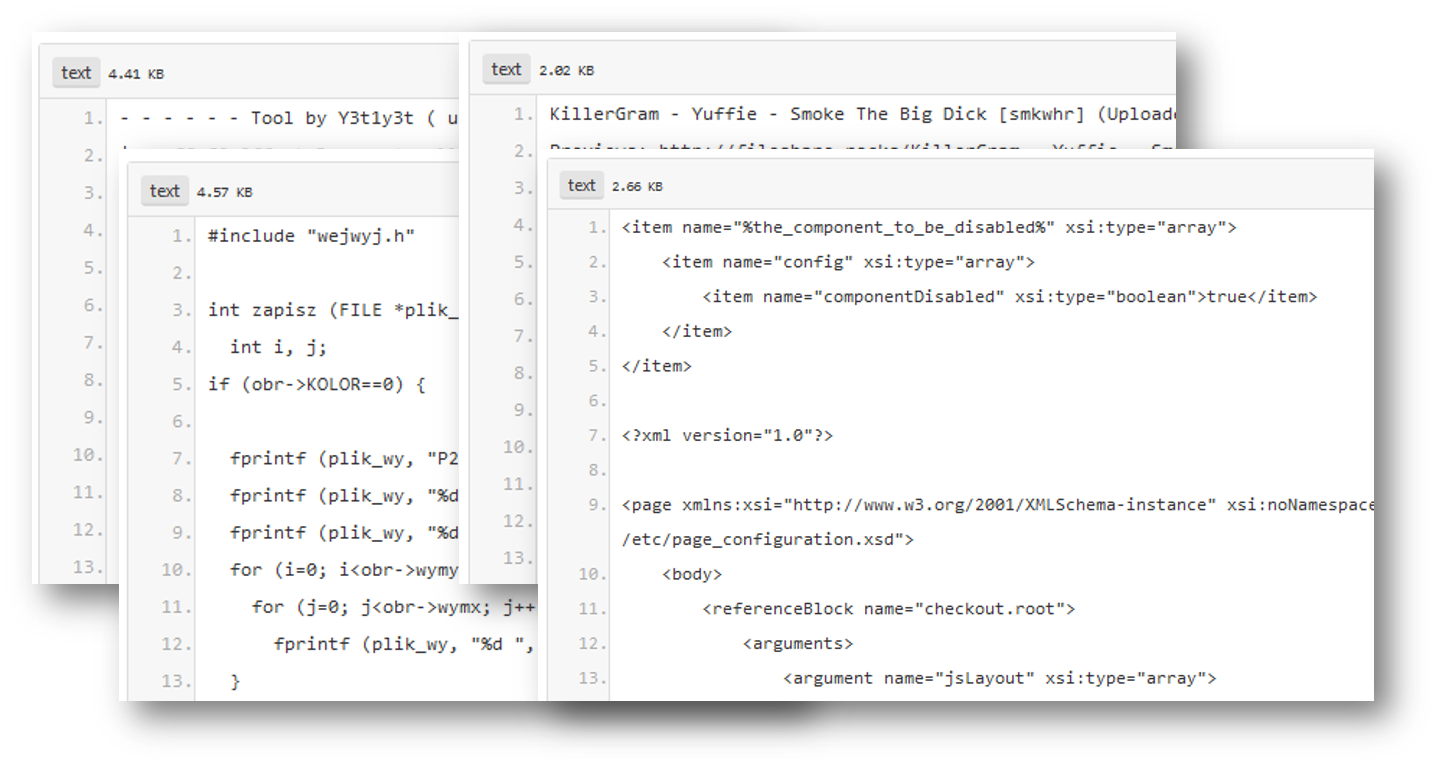
\includegraphics[scale=0.32, angle=0]{images/pastes-ex.png}
    \end{figure}
\end{frame}

\begin{frame}
    \frametitle{Sources of leaks: Others}
        \begin{itemize}
            \item Mistakes from users
            \begin{itemize}
                \item \tiny{https://github.com/}\normalsize{search?q=remove\_password}\tiny{\&type=Commits\&ref=searchresults}
            \end{itemize}
            \begin{figure}
                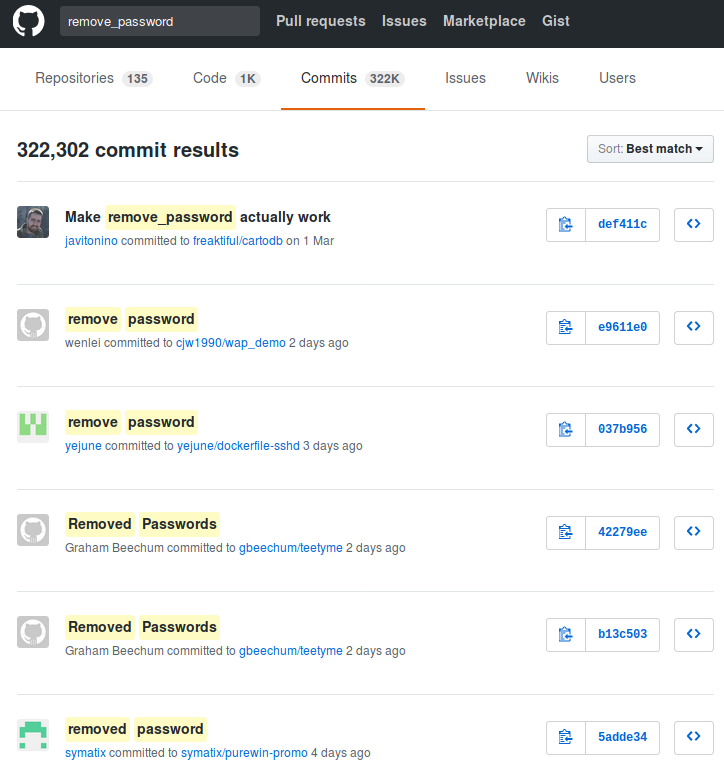
\includegraphics[scale=0.4]{images/git-pass.png}
            \end{figure}
        \end{itemize}
\end{frame}

\begin{frame}
    \frametitle{Sources of leaks: Others}
        \begin{itemize}
            \item Mistakes from users
            \begin{itemize}
                \item \tiny{https://github.com/}\normalsize{search?q=remove\_password}\tiny{\&type=Commits\&ref=searchresults}
            \end{itemize}
            \begin{figure}
                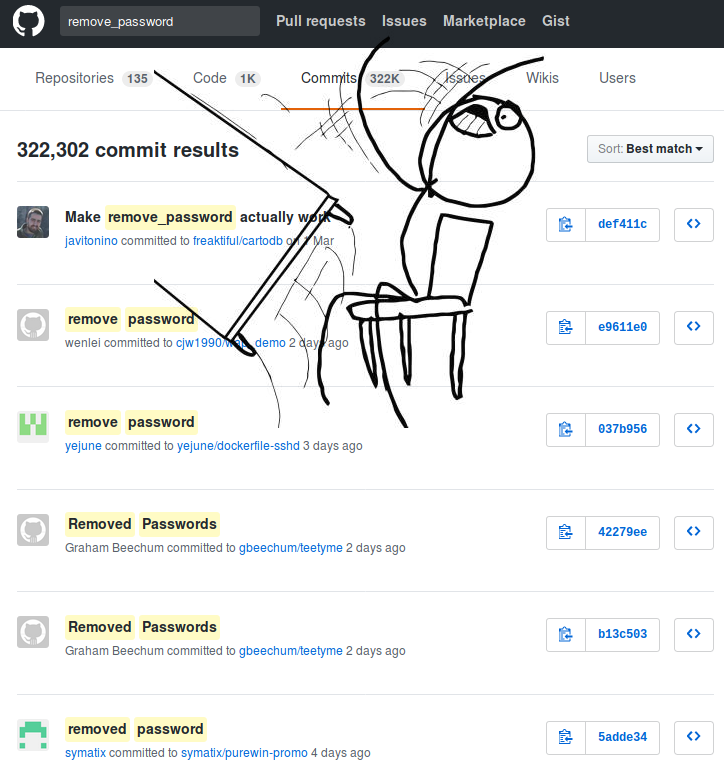
\includegraphics[scale=0.4]{images/git-pass-table.png}
            \end{figure}
        \end{itemize}
\end{frame}

\begin{frame}
        \frametitle{Why so many leaks?}
        \begin{itemize}
                \item Economical interests (e.g. Adversaries promoting services)
                \item Political motives (e.g. Adversaries showing off)
                \item Collaboration (e.g. Criminals need to collaborate)
                \item Operational infrastructure (e.g. malware exfiltrating information on a pastie website)
                \item Mistakes and Errors
        \end{itemize}
\end{frame}


\begin{frame}
    \frametitle{Are leaks frequent?}
    \begin{center}
    \Large{Yes!}\\ and we have to deal with this as a CSIRT.
    \end{center}

    \begin{itemize}
            \item {\bf Contacting companies or organisations} who did specific accidental leaks
            \item {\bf Discussing with media} about specific case of leaks and how to make it more practical/factual for everyone
            \item Evaluating the economical market for cyber criminals (e.g. DDoS booters\footnote{\url{https://github.com/D4-project/}} or reselling personal information - reality versus media coverage)
            \item Analysing collateral effects of malware, software vulnerabilities or exfiltration
    \end{itemize}

    \begin{center}
    $\rightarrow$ And it's important to detect them automatically.
    \end{center}
\end{frame}

\begin{frame}
    \frametitle{Paste monitoring at CIRCL: Statistics}
    \begin{itemize}
        \item Monitored paste sites: 27
            \begin{itemize}
                \item \textit{pastebin.com}
                \item \textit{ideone.com}
                \item \textit{...}
            \end{itemize}
    \end{itemize}
    \begin{table}[h]
    \centering
    \begin{tabular}{|lrrr|}
        \hline
        \rowcolor{lightgray} & 2016 & 2017 & 08.2018\\
        Collected pastes & 18,565,124 & 19,145,300 & 11,591,987 \\
        Incidents & 244 & 266 & 208\\
        \hline
    \end{tabular}
    \caption{Pastes collected and incident\footnote{\url{http://www.circl.lu/pub/tr-46}} raised by CIRCL}
    \label{circlStats}
\end{table}

\end{frame}

\begin{frame}
        \frametitle{Privacy, AIL and GDPR}
        \begin{itemize}
                \item Many modules in AIL can process personal data and even special categories of data as defined in GDPR (Art. 9).
                \item The data controller is often the operator of the AIL framework (limited to the organisation) and has to define {\bf legal grounds for processing personal data}.
                \item To help users of AIL framework, a document is available which describe points of AIL in regards to the regulation\footnote{\url{https://www.circl.lu/assets/files/inform
ation-leaks-analysis-and-gdpr.pdf}}.
        \end{itemize}
\end{frame}

\begin{frame}
        \frametitle{Potential legal grounds}
        \begin{itemize}
                \item {\bf Consent of the data subject} is in many cases not feasible in practice and often impossible or illogical to obtain (Art. 6(1)(a)).
                \item Legal obligation (Art. 6(1)(c)) - This legal ground applies mostly to CSIRTs, in accordance with the powers and responsibilities set out in CSIRTs mandate and with their constituency, as they may have the legal obligation to collect, analyse and share information leaks without having a prior consent of the data subject.
				\item Art. 6(1)(f) - Legitimate interest - Recital 49 explicitly refers to CSIRTs’ right to process personal data provided that they have a legitimate interest but not colliding with fundamental rights and freedoms of data subject.
        \end{itemize}
\end{frame}


\section{AIL Framework}
% AIL EXPLANATION
\begin{frame}
    \frametitle{From a requirement to a solution: AIL Framework}
    \large{History:}
    \begin{itemize}
        \item AIL initially started as an \textbf{internship project} (2014) to evaluate the feasibility to automate the analysis of (un)structured information to find leaks.
        \item In 2019, AIL framework is an \textbf{open source software} in Python. The software is actively used (and maintained) by CIRCL.
    \end{itemize}
\end{frame}

\begin{frame}
    \frametitle{AIL Framework: A framework for Analysis of Information Leaks}
    \begin{quote}
"AIL is a modular framework to analyse potential information leaks from unstructured data sources like pastes from Pastebin."
    \end{quote}
    \vskip0.5cm

    \begin{tikzpicture}[scale=1.0]
        \tikzstyle{flux}=[->,>=latex, thick]

        \tikzstyle{node}=[circle,draw, align=center]
        \tikzstyle{rect}=[rectangle,draw, align=center]
        \tikzstyle{simplenode}=[align=center]

        \node[simplenode] (pastebin) at (0, 0) {
\includegraphics[scale=0.20]{images/pastebin.png}};
        \node[simplenode] (leaks) at (4, -2) {Other leaks};
        \node[simplenode] (ail) at (4, 0) {
\includegraphics[scale=0.3]{images/circl-small.png}};
        \node[simplenode] (res) at (8, 0) {
\includegraphics[scale=0.1]{images/alert.png}};

        \begin{scope}
            \draw[flux] (pastebin.east) to (ail.west);
        \foreach \i in {-2,...,-1}{% 
            \pgfmathsetlengthmacro{\radius}{(sin(atan(\i*0.1))+0.1)*1cm}
            %\draw[->] ([yshift=\i * 0.2 cm]pastebin.east) to [out=-50,in=-130] ([yshift=\i * 0.2 cm]ail.west) ;}
            %\draw[->] ([xshift=\radius,yshift=\i * 0.2 cm]pastebin.east) to [out=-10+\i*10,in=-130] ([yshift=\i * 0.2 cm]ail.west) ;}
            \draw[flux] ([xshift=\radius,yshift=\i * 0.2 cm]pastebin.east) to [out=-10+\i*10,in=-130] ([xshift=-\i*0.05cm,yshift=\i * 0.2 cm]ail.west) ;}

        \foreach \i in {1,...,3}{% 
            \pgfmathsetlengthmacro{\radius}{(sin(atan(\i*0.1))-0.1)*1cm}
            \draw[flux] ([xshift=-\radius,yshift=\i * 0.2 cm]pastebin.east) to [out=10+\i*10,in=130] ([xshift=\i*0.05cm,yshift=\i * 0.2 cm]ail.west) ;}
        \draw[->,>=latex, very thick] (ail) to (res);
        \draw[->,>=latex, very thick] (leaks) to (ail);
        \end{scope}


    \end{tikzpicture}
\end{frame}



\begin{frame}
    \frametitle{AIL Framework: Current capabilities}
    \begin{itemize}
        \item Extending AIL to add a new {\bf analysis module} can be done in 50 lines of Python
        \item The framework {\bf supports multi-processors/cores by default}. Any analysis module can be started multiple times to support faster processing during peak times or bulk import
        \item \textbf{Multiple} concurrent \textbf{data input}
        \item Tor Crawler
    \end{itemize}
\end{frame}

\begin{frame}
    \frametitle{AIL Framework: Current features}
    \begin{itemize}
        \item Extracting \textbf{credit cards numbers, credentials, phone numbers, ...}
        \item Extracting and validating potential \textbf{hostnames}
        \item Keeps track of \textbf{duplicates}
        \item Submission to threat sharing and incident response platform (\textbf{MISP} and \textbf{TheHive})
        \item \textbf{Full-text indexer} to index unstructured information
        \item \textbf{Tagging} for classification and searches
        \item Terms, sets and regex \textbf{tracking and occurences}
        \item Archives, files and raw \textbf{submission} from the UI
        \item PGP and Decoded (Base64, ...) Correlation
        \item And many more
    \end{itemize}
\end{frame}

\section{Live demo!}

\begin{frame}
    \frametitle{Example: Dashboard}
    \begin{figure}
        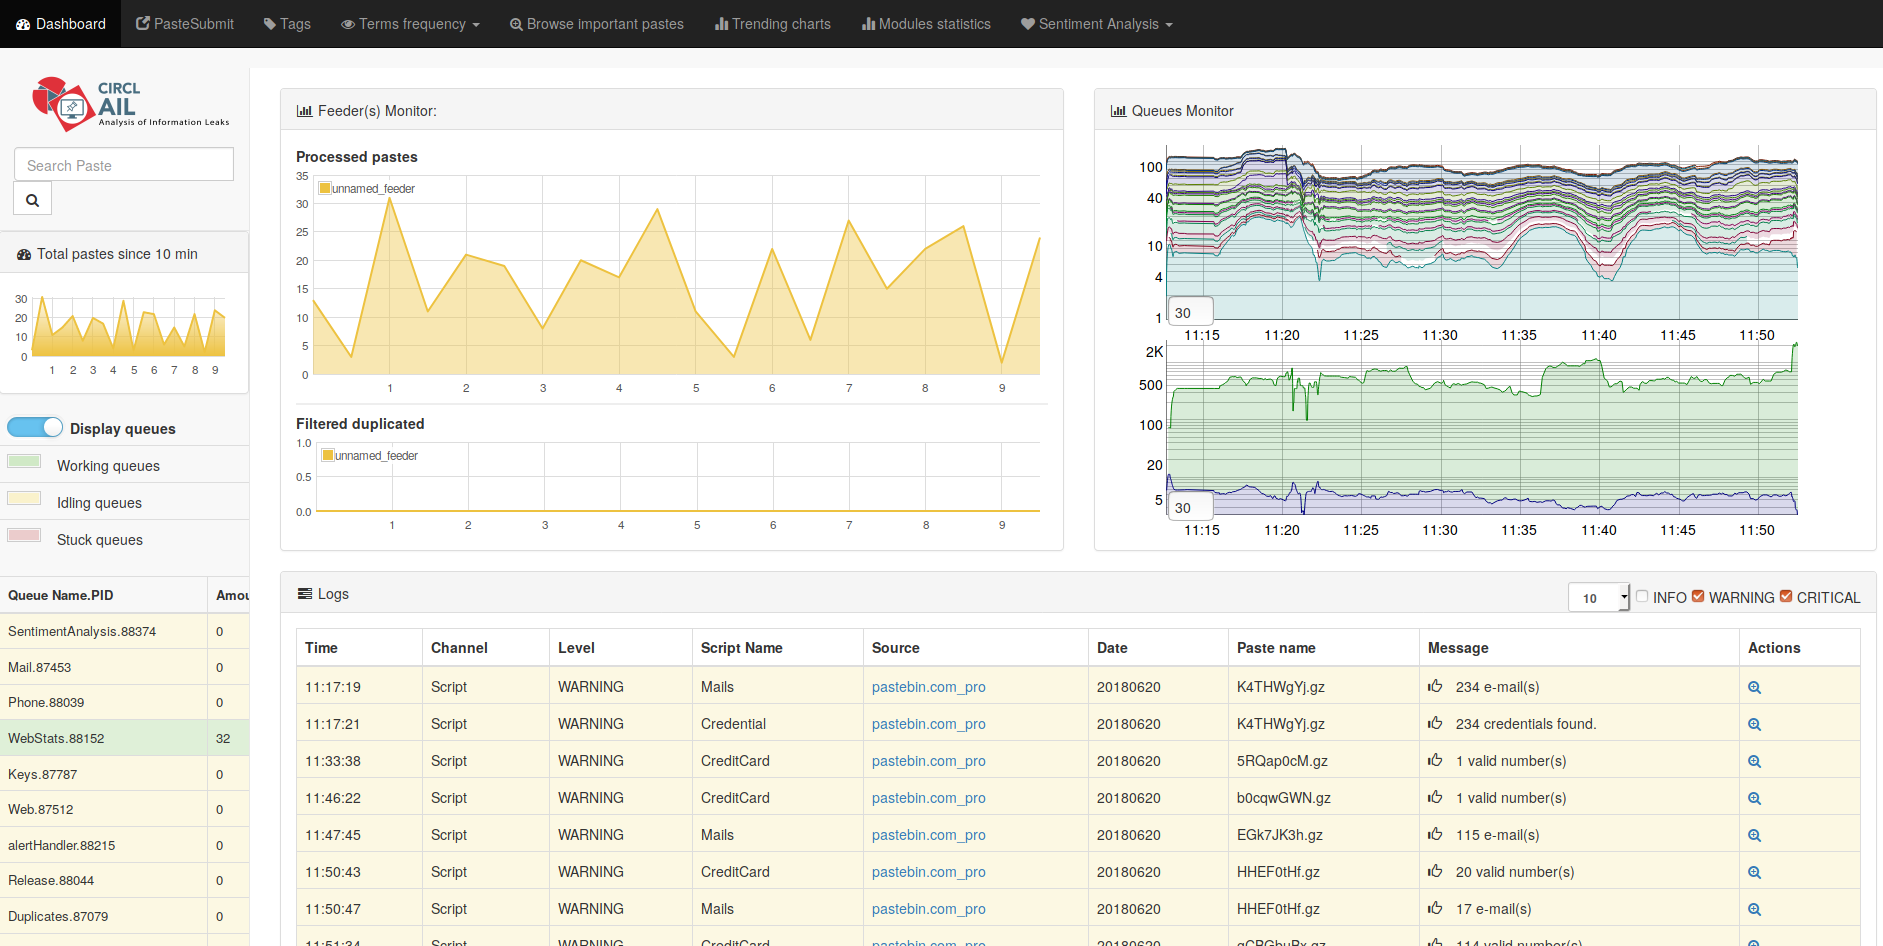
\includegraphics[scale=0.18, angle=0]{screenshot/dashboard.png}
    \end{figure}
\end{frame}


\begin{frame}
    \frametitle{Example: Text search}
    \begin{figure}
        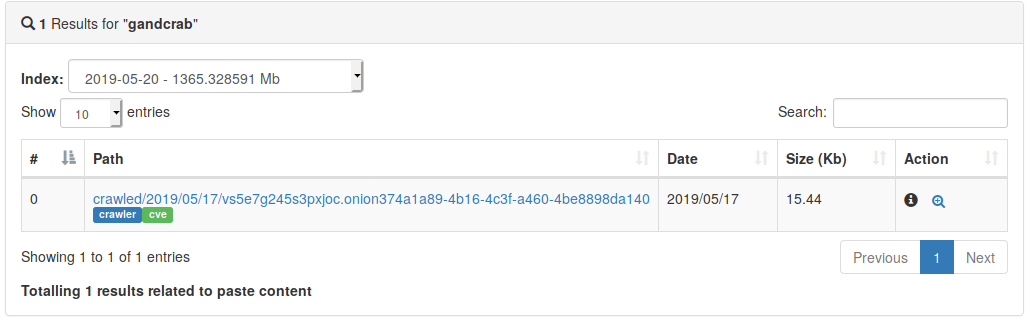
\includegraphics[scale=0.3, angle=0]{images/ail_02.png}
    \end{figure}
\end{frame}

\begin{frame}
    \frametitle{Example: Pastes Metadata (1)}
    \begin{figure}
        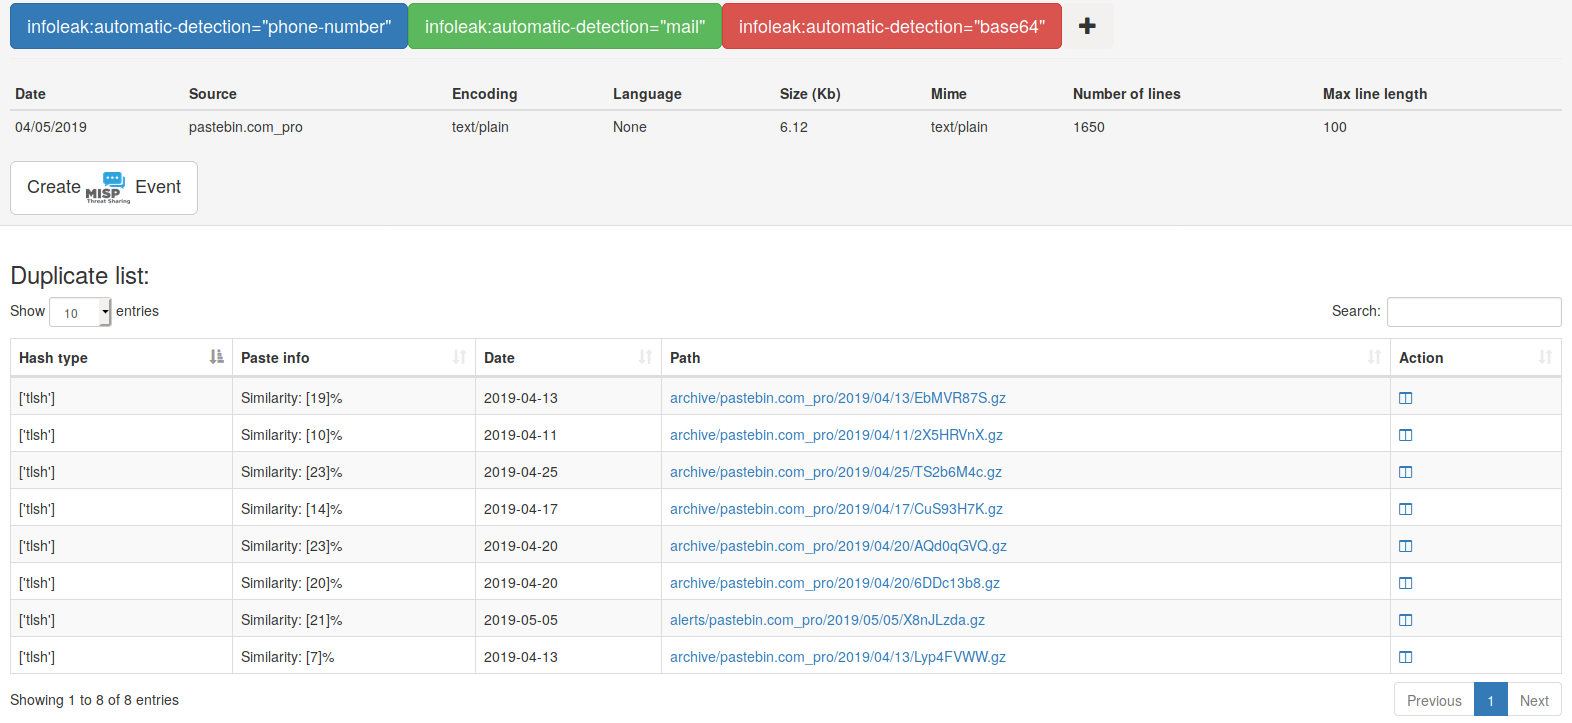
\includegraphics[scale=0.21, angle=0]{images/ail_15.png}
    \end{figure}
\end{frame}

\begin{frame}
    \frametitle{Example: Pastes Metadata (2)}
    \begin{figure}
        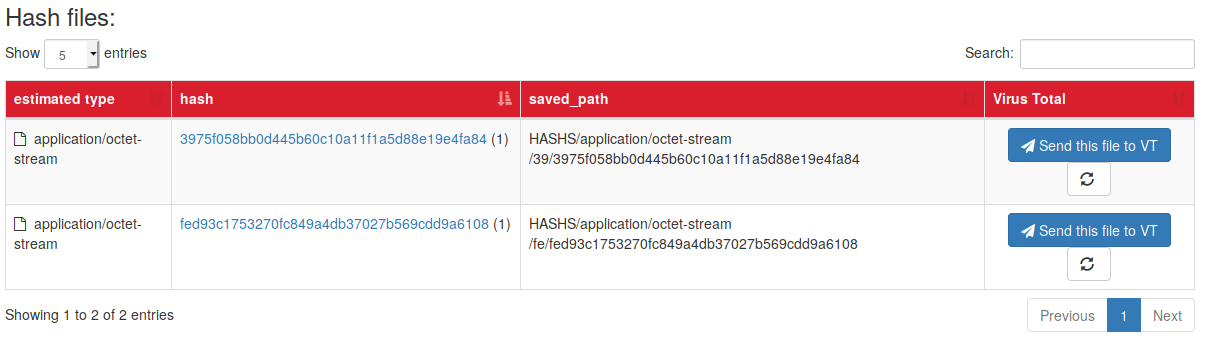
\includegraphics[scale=0.28, angle=0]{images/ail_16.png}
    \end{figure}
\end{frame}

\begin{frame}
    \frametitle{Example: Pastes Metadata (3)}
    \begin{figure}
        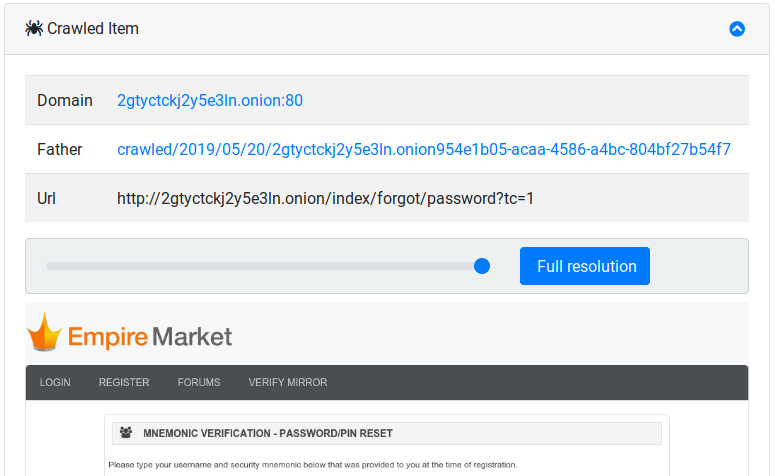
\includegraphics[scale=0.28, angle=0]{images/ail_17.png}
    \end{figure}
\end{frame}

\begin{frame}
    \frametitle{Example: Browsing content}
    \begin{figure}
        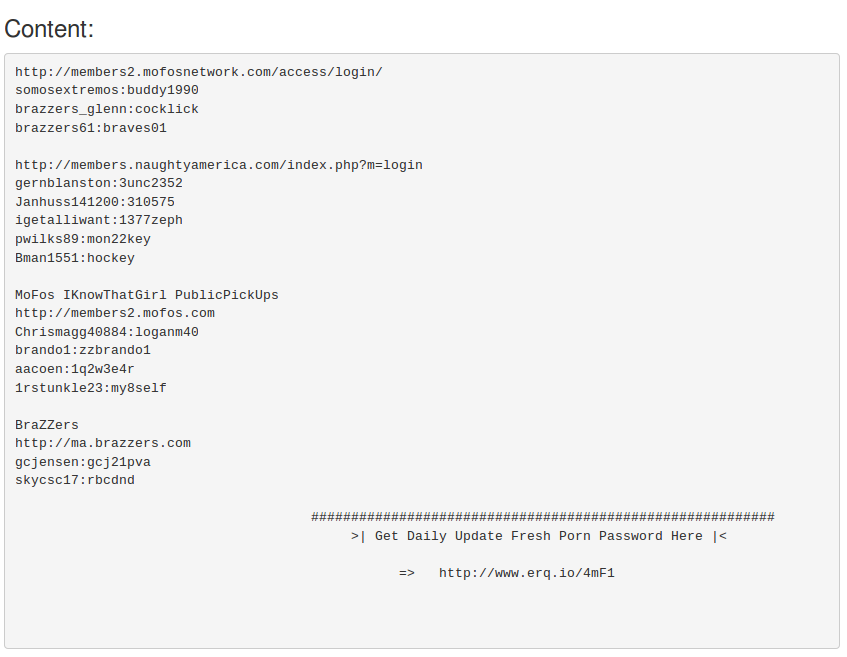
\includegraphics[scale=0.3, angle=0]{images/ail_04.png}
    \end{figure}
\end{frame}


\begin{frame}
    \frametitle{Example: Browsing content}
    \begin{figure}
        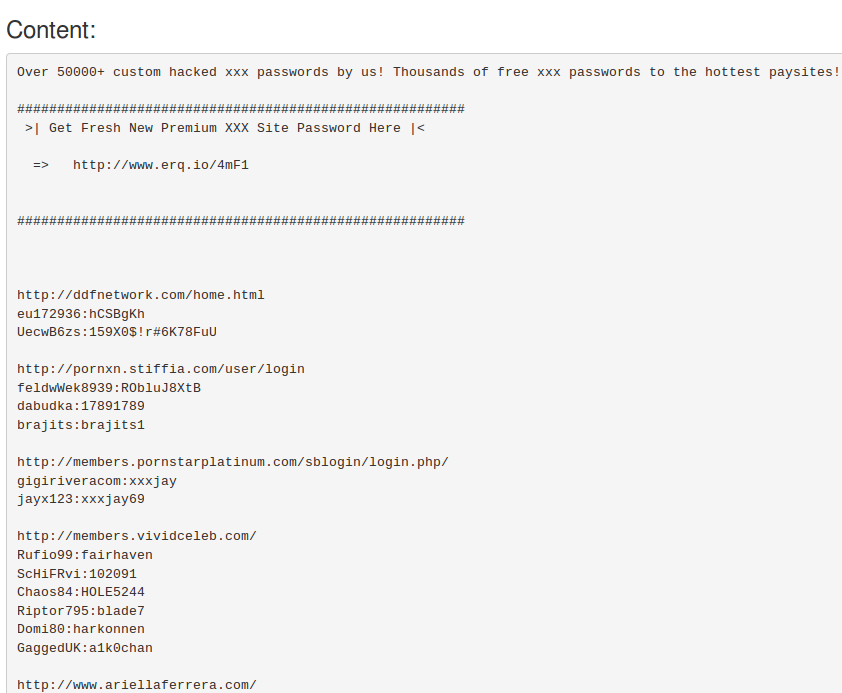
\includegraphics[scale=0.3, angle=0]{images/ail_06.png}
    \end{figure}
\end{frame}

\begin{frame}
    \frametitle{Example: Search by tags}
    \begin{figure}
        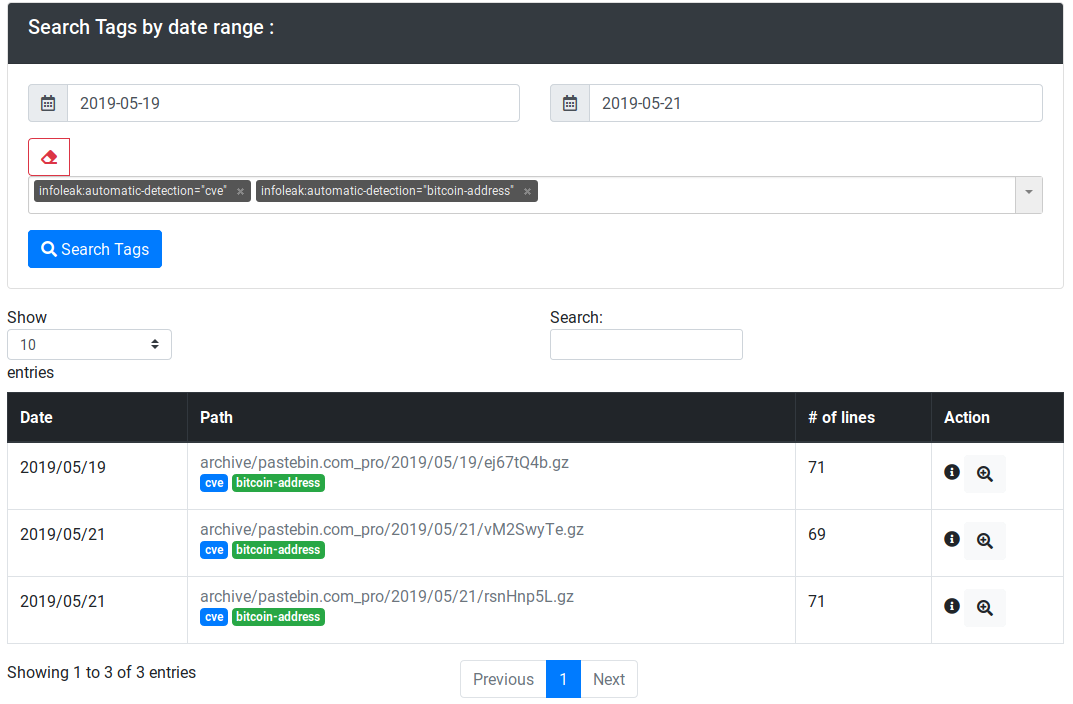
\includegraphics[scale=0.26, angle=0]{images/ail_14.png}
    \end{figure}
\end{frame}

%%%
%%%
%%%

%\begin{frame}
%    \centerline{
\includegraphics[scale=0.35]{images/uncle-sam.jpg}}
%\end{frame}

% INSTALLATION
\section{Setting up the framework}
\lstset{style=bash}
\begin{frame}[fragile]
    \frametitle{Setting up AIL-Framework from source or virtual machine}
\vspace{-0.2cm}
    \begin{tcblisting}{colback=black!85,coltext=green,listing only,
        title=Setting up AIL-Framework from source, fonttitle=\bfseries}
git clone https://github.com/CIRCL/AIL-framework.git
cd AIL-framework
./installing_deps.sh
cd var/www/
./update_thirdparty.sh
\end{tcblisting}
\vspace{-0.2cm}
Using the virtual machine:
\begin{enumerate}
    \item Download from CIRCL website\footnote{\url{https://www.circl.lu/assets/files/ail-training/AIL\_v@4986352.ova}} or use the provided USB key
    \item Start virtualbox
    \item File $\rightarrow$ import appliance $\rightarrow$ select AIL\_June.ova
    \item Automatic update handled by the launcher
\end{enumerate}
\end{frame}

% AIL ecosystem: Challenges and design
\section{AIL ecosystem - Challenges and design}
\begin{frame}
    \frametitle{AIL ecosystem: Technologies used}
    \begin{itemize}
        \item[] \textbf{Programing language:} Full python3
        \item[] \textbf{Databases:} Redis and ARDB
        \item[] \textbf{Server:} Flask
        \item[] \textbf{Data message passing:} ZMQ, Redis list and Redis Publisher/Subscriber
    \end{itemize}
\end{frame}

\begin{frame}[fragile]
    \textbf{\large AIL global architecture 1/2}\\

    \begin{figure}
        \centering
        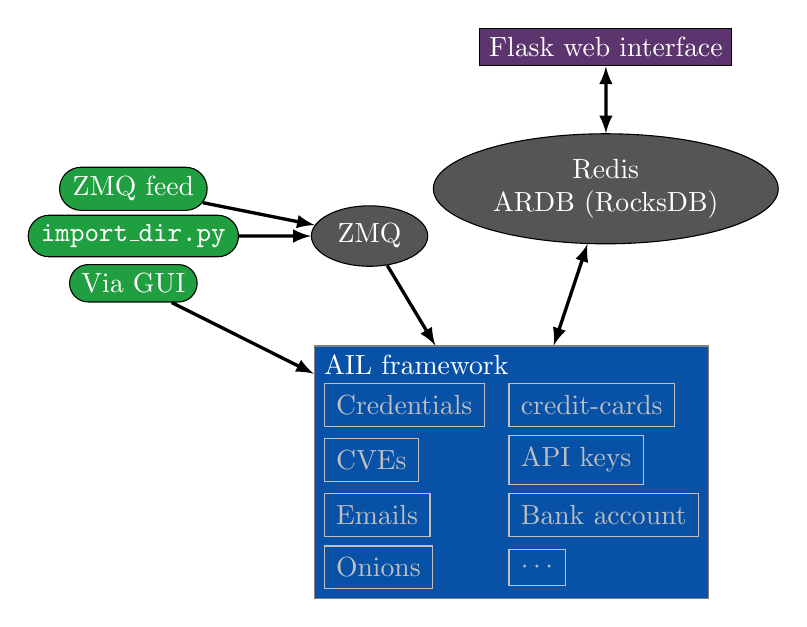
\begin{tikzpicture}[scale=1.2]
        %styles
        \tikzstyle{mymatrix}=[matrix of nodes, nodes=typetag, row sep=0.3em, draw=gray, fill={rgb:red,0.04;green,0.43;blue,0.89}]
        \tikzstyle{mycontainer}=[draw=gray, inner sep=1ex]
        \tikzstyle{typetag}=[draw=gray, inner sep=1ex, anchor=west, color=lightgray]
        \tikzstyle{title}=[draw=none, color=white, inner sep=0pt]
    
        \tikzstyle{feeder}=[rounded rectangle,draw, align=center, fill={rgb:red,1;green,5;blue,2}]
        \tikzstyle{ail}=[rectangle,draw, align=center, fill={rgb:red,0.04;green,0.43;blue,0.89}]
        \tikzstyle{ail2}=[rectangle,draw, align=center, fill={rgb:red,0.74;green,0.43;blue,0.89}]
        \tikzstyle{storage}=[ellipse,draw, align=center, fill={rgb:red,3;green,3;blue,3}]
        \tikzstyle{commu}=[->,>=latex,very thick]
        \tikzstyle{commuboth}=[<->,>=latex,very thick]
    
        %nodes
        \node[feeder] (f1) at (0,0) {\color{white}ZMQ feed};
        \node[feeder] (f2) at (0,-0.5) {\color{white}\texttt{import\_dir.py}};
        \node[feeder] (f3) at (0,-1) {\color{white}Via GUI};
    
        \node[storage] (st1) at (2.5,-0.5) {\color{white}ZMQ};
    
        \matrix[mymatrix] (a2) at (4,-3) {
            |[title]|AIL framework\\
            Credentials & credit-cards\\
            CVEs & API keys\\
            Emails & Bank account\\
            Onions & $\cdots$\\
        };
    
        \node[storage] (st2) at (5,0) {\color{white}Redis\\\color{white}ARDB (RocksDB)};
        \node[ail2] (a3) at (5,1.5) {\color{white}Flask web interface};
        
        %arraws
        \draw[commu] (f1)--(st1);
        \draw[commu] (f2)--(st1);
        \draw[commu] (f3)--(a2);
    
        \draw[commu] (st1)--(a2);
    
        \draw[commuboth] (a2)--(st2);
    
        \draw[commuboth] (st2)--(a3);
        
        \end{tikzpicture}
    \end{figure}
\end{frame}

\begin{frame}
    \textbf{\large AIL global architecture 2/2}\\
    {\tiny Redis PubSub 1: port 6380, channel queuing}\\
    \vskip -0.5em
    {\tiny Redis PubSub 2: port 6380, channel script}
    
    \begin{center}
    \vskip -2.0em
    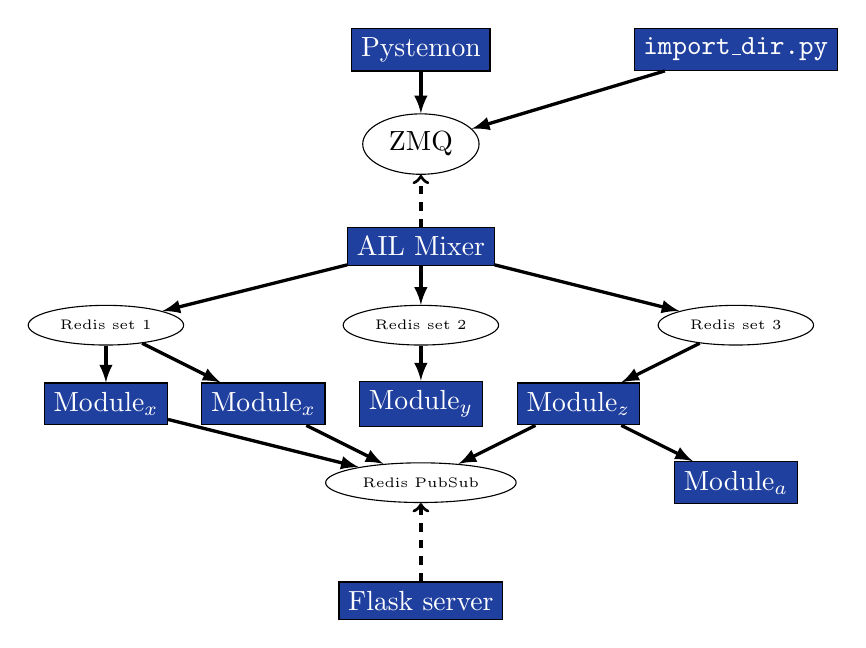
\begin{tikzpicture}[scale=1.0]
    %styles
    \tikzstyle{queue}=[ellipse,draw,align=center]
    \tikzstyle{module}=[rectangle,draw, align=center, fill={rgb:red,1;green,2;blue,5}]
    \tikzstyle{commu}=[->,>=latex,very thick]
    \tikzstyle{subs}=[->,dashed,very thick]
    %nodes
    \node[module] (py) at (0,0.5) {\color{white}Pystemon};
    \node[module] (imp) at (4,0.5) {\color{white}\texttt{import\_dir.py}};
    \node[queue] (zmq) at (0,-0.7) {ZMQ};
    \node[module] (ail) at (0,-2) {\color{white}AIL Mixer};
    \node[queue] (rps1) at (-4,-3) {\tiny Redis set 1};
    \node[queue] (rps2) at (0,-3) {\tiny Redis set 2};
    \node[queue] (rps3) at (4,-3) {\tiny Redis set 3};
    \node[module] (m1) at (-2,-4) {\color{white}Module$_x$};
    \node[module] (m4) at (-4,-4) {\color{white}Module$_x$};
    \node[module] (m2) at (0,-4) {\color{white}Module$_y$};
    \node[module] (m3) at (2,-4) {\color{white}Module$_z$};
    \node[queue]  (rps4) at (0,-5) {\tiny Redis PubSub};
    \node[module] (ma) at (4,-5) {\color{white}Module$_a$};
    \node[module] (flask) at (0,-6.5) {\color{white}Flask server};
    
    %arraws
    \draw[commu] (py)--(zmq);
    \draw[commu] (imp)--(zmq);
    \draw[subs]  (ail)--(zmq);
    \draw[commu] (ail)--(rps1);
    \draw[commu] (ail)--(rps2);
    \draw[commu] (ail)--(rps3);
    \draw[commu] (rps1)--(m1);
    \draw[commu] (rps1)--(m4);
    \draw[commu] (rps2)--(m2);
    \draw[commu] (rps3)--(m3);
    \draw[commu] (m1)--(rps4);
    \draw[commu] (m4)--(rps4);
    \draw[commu] (m3)--(rps4);
    \draw[commu]  (m3)--(ma);
    \draw[subs]  (flask)--(rps4);

    \end{tikzpicture}
    \end{center}

\end{frame}

\begin{frame}
    \frametitle{Data feeder: Gathering pastes with pystemon}
    \textbf{\large Pystemon global architecture}\\
    {\tiny Redis PubSub 1: port 6380, channel queuing}\\
    \vskip -0.5em
    {\tiny Redis PubSub 2: port 6380, channel script}
    
    \begin{center}
    %\vskip -2.0em
    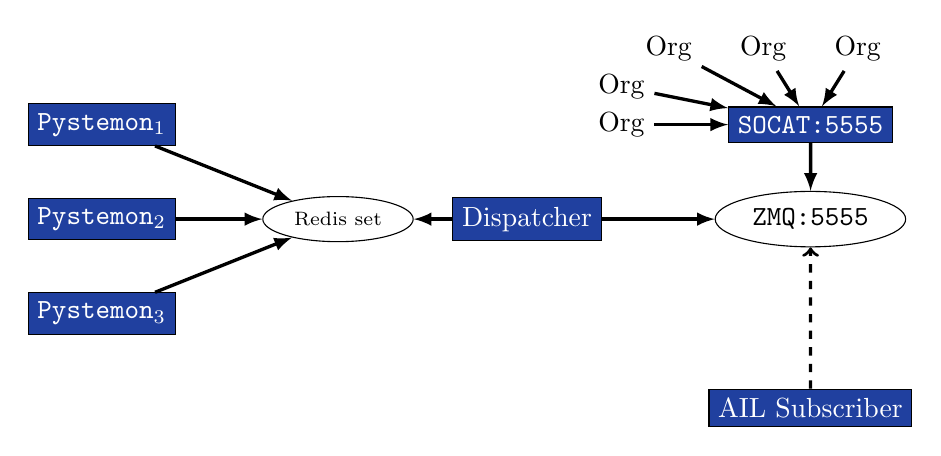
\begin{tikzpicture}[scale=1.2]
    %styles
    \tikzstyle{queue}=[ellipse,draw,align=center]
    \tikzstyle{module}=[rectangle,draw, align=center, fill={rgb:red,1;green,2;blue,5}]
    \tikzstyle{commu}=[->,>=latex,very thick]
    \tikzstyle{subs}=[->,dashed,very thick]
    %nodes
    \node[module] (py1) at (-0.5,1) {\color{white}\texttt{Pystemon$_1$}};
    \node[module] (py2) at (-0.5,0) {\color{white}\texttt{Pystemon$_2$}};
    \node[module] (py3) at (-0.5,-1) {\color{white}\texttt{Pystemon$_3$}};
        \node[queue] (red) at (2,0) {{\scriptsize Redis set}};
    \node[module] (dis) at (4,0) {\color{white}Dispatcher};
    \node[queue] (zmq) at (7,0) {\texttt{ZMQ:5555}};
    \node[module] (soc) at (7,1) {\color{white}\texttt{SOCAT:5555}};
    \node[module] (ail) at (7,-2) {\color{white}AIL Subscriber};

    \node (c1) at (5.5,1.8) {Org};
    \node (c2) at (5,1.4) {Org};
    \node (c3) at (5,1)   {Org};
    \node (c4) at (6.5,1.8) {Org};
    \node (c5) at (7.5,1.8) {Org};


    %arraws
    \draw[commu] (py1)--(red);
    \draw[commu] (py2)--(red);
    \draw[commu] (py3)--(red);
    \draw[commu] (dis)--(red);
    \draw[commu] (dis)--(zmq);
    \draw[commu] (soc)--(zmq);
    \draw[subs] (ail)--(zmq);

    \draw[commu] (c1)--(soc);
    \draw[commu] (c2)--(soc);
    \draw[commu] (c3)--(soc);
    \draw[commu] (c4)--(soc);
    \draw[commu] (c5)--(soc);

    \end{tikzpicture}
    \end{center}


\end{frame}


\begin{frame}
    \frametitle{AIL global architecture: Data streaming between module}
    \centerline{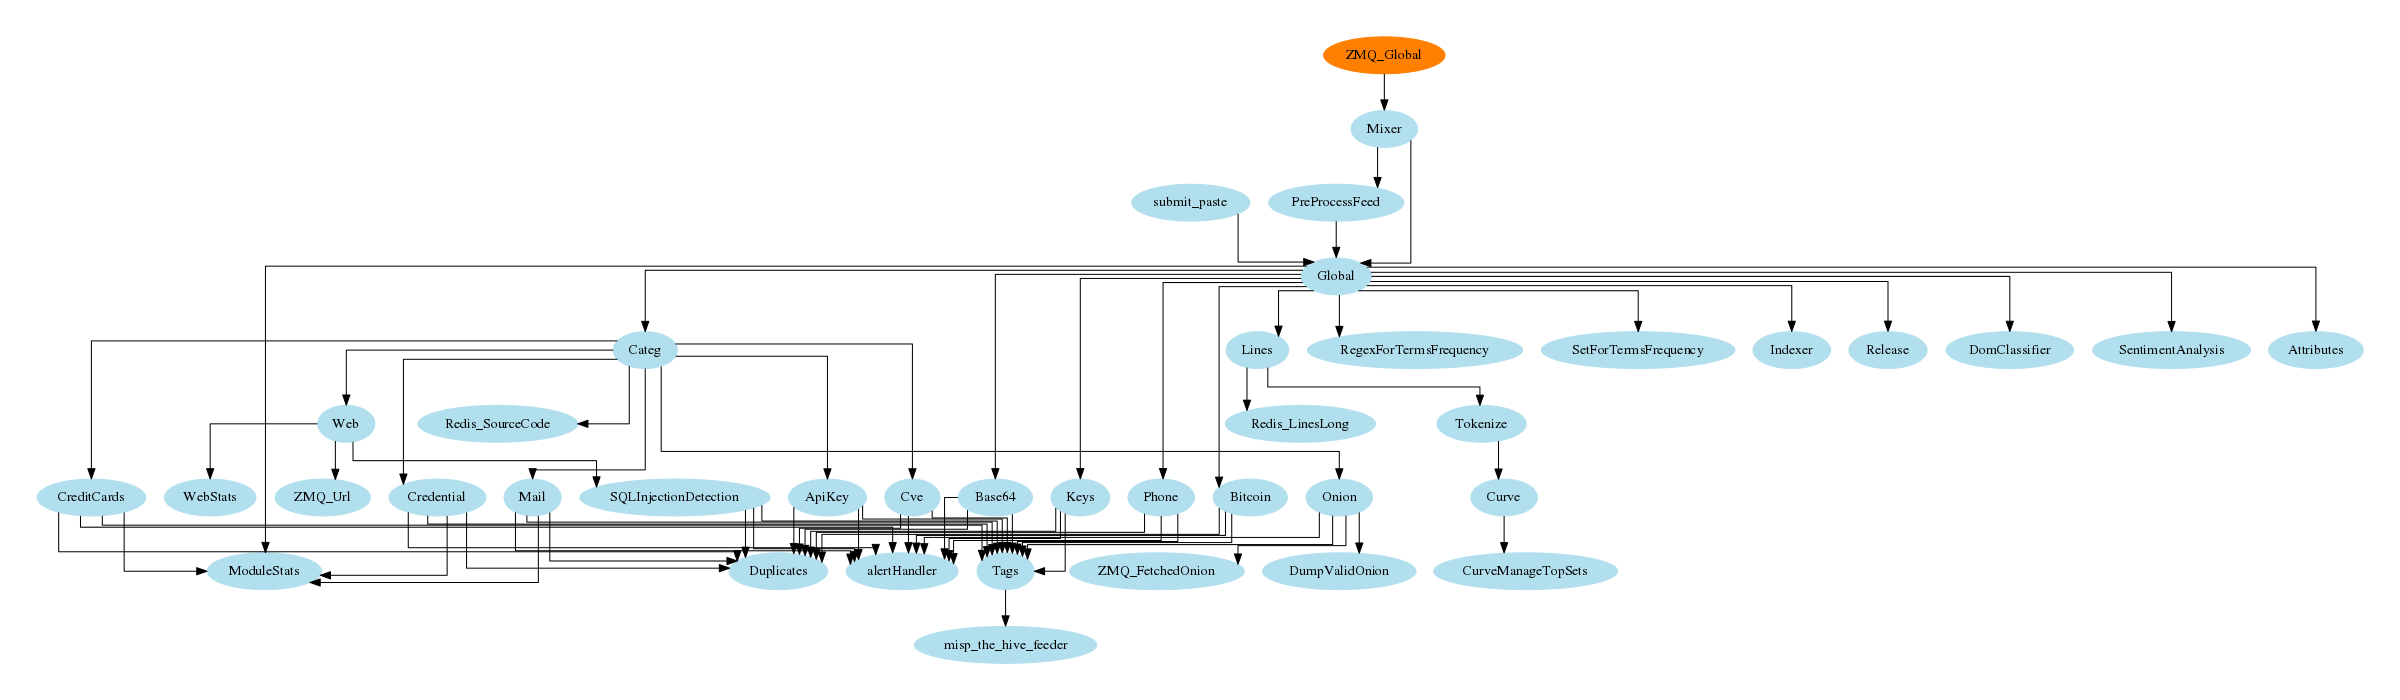
\includegraphics[scale=0.15]{images/module-data-flow.png}}
\end{frame}

\begin{frame}
    \frametitle{AIL global architecture: Data streaming between module (Credential example)}
    \centerline{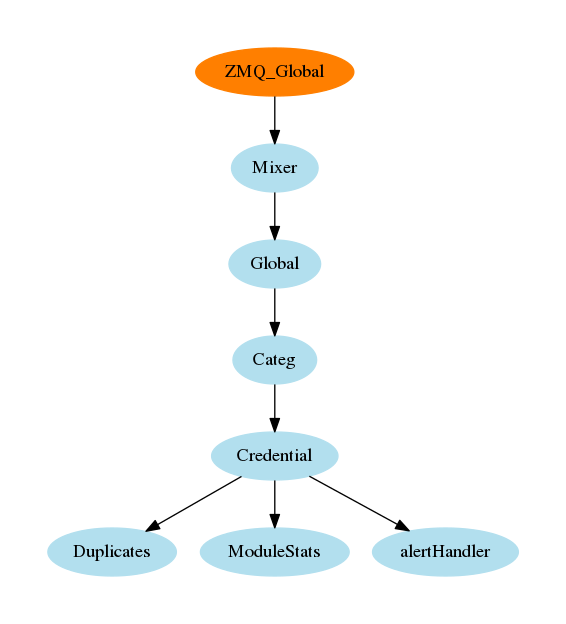
\includegraphics[scale=0.31]{images/stream_exemp_cred.png}}
\end{frame}

\begin{frame}
    \frametitle{Message consuming}
    \begin{center}
    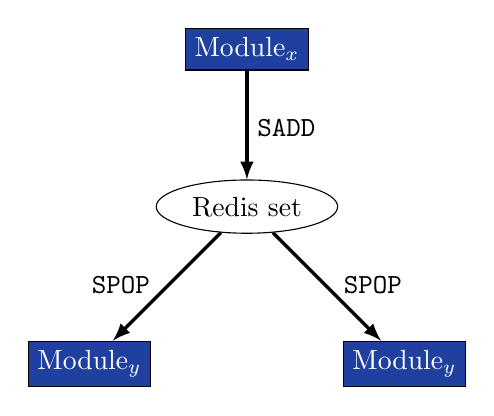
\begin{tikzpicture}[scale=1.0]
    %styles
    \tikzstyle{queue}=[ellipse,draw,align=center]
    \tikzstyle{module}=[rectangle,draw, align=center, fill={rgb:red,1;green,2;blue,5}]
    \tikzstyle{commu}=[->,>=latex,very thick]
    %nodes
    \node[module] (m0) at (0,2) {\color{white}Module$_x$};
    \node[queue] (rps1) at (0,0) {Redis set};
    \node[module] (m1) at (-2,-2) {\color{white}Module$_y$};
    \node[module] (m2) at (2,-2) {\color{white}Module$_y$};

    \node (t1) at (-1.6,-1) {\texttt{SPOP}};
    \node (t2) at (1.6,-1) {\texttt{SPOP}};
    \node (t3) at (0.5,1) {\texttt{SADD}};
    
    %arraws
    \draw[commu] (m0)--(rps1);
    \draw[commu] (rps1)--(m1);
    \draw[commu] (rps1)--(m2);

    \end{tikzpicture}


    \vskip 1em
    \begin{itemize}
        \item[] $\rightarrow$ No message lost nor double processing
        \item[] $\rightarrow$ Multiprocessing!
    \end{itemize}
    \end{center}
\end{frame}

\begin{frame}
        \frametitle {Web crawler}
        \begin{itemize}
                \item Web crawler is used to crawl regular website as well as .onion addresses
                \item Splash (scriptable browser) is rending the pages (including javascript) and produce screenshots (HAR archive too)
        \end{itemize}
\begin{figure}[h] 
    \centering 
    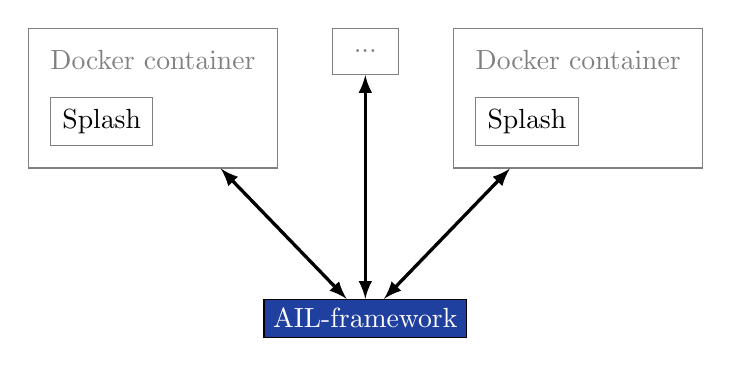
\begin{tikzpicture}[scale=1.0, 
        mymatrix/.style={matrix of nodes, nodes=typetag, row sep=1em}, 
        mycontainer/.style={draw=gray, inner sep=1ex}, 
        typetag/.style={draw=gray, inner sep=1ex, anchor=west}, 
        title/.style={draw=none, color=gray, inner sep=0pt} 
    ] 
 
    %styles 
    \tikzstyle{Docker}=[ellipse,draw,align=center] 
    \tikzstyle{AIL}=[rectangle,draw, align=center, fill={rgb:red,1;green,2;blue,5}] 
    \tikzstyle{Splash}=[rectangle,draw, align=center, fill={rgb:red,1;green,2;blue,5}] 
    \tikzstyle{commu}=[<->,>=latex,very thick] 
 
    %nodes 
    \matrix[mymatrix] (mx1) at (0, 0) { 
        |[title]|Docker container \\ 
        Splash \\ 
    }; 
    \matrix[mymatrix, right=of mx1.north east, matrix anchor=north west] (mx2) { 
    %\matrix[mymatrix] (mx2) at (1, 0) { 
        |[title]|... \\ 
    }; 
    \matrix[mymatrix, right=of mx2.north east, matrix anchor=north west] (mx3) { 
    %\matrix[mymatrix] (mx3) (2, 0){ 
        |[title]|Docker container \\ 
        Splash \\ 
    }; 
 
    \node[mycontainer, fit=(mx1)] (c1) {}; 
    \node[mycontainer, fit=(mx2)] (c2) {}; 
    \node[mycontainer, fit=(mx3)] (c3) {}; 
 
    %\node[AIL, below=of mx2.south, matrix anchor=north] (ail) {\color{white}AIL-framework}; 
    \node[AIL, below= 3cm of mx2.south, matrix anchor=north] (ail) {\color{white}AIL-framework}; 
 
    %arraws 
    \draw[commu] (ail)--(c1); 
    \draw[commu] (ail)--(c2); 
    \draw[commu] (ail)--(c3); 
 
 
    \end{tikzpicture} 
    \caption{Architecture of AIL and its hidden services crawler} 
    \label{crawler-schema} 
\end{figure} 
\end{frame}

%STARTING THE SYSTEM
\section{Starting the framework}
\lstset{style=bash}
\begin{frame}[fragile]
    \frametitle{Running your own instance from source}
    {\scriptsize Make sure that ZMQ\_Global$\rightarrow$address = \texttt{tcp://crf.circl.lu:5556,tcp://127.0.0.1:5556} in bin/package/config.cfg}
    \begin{tcblisting}{colback=black!85,coltext=green,listing only,
        title=Accessing the environment and starting AIL, fonttitle=\bfseries}
# Activate the virtualenv
. ./AILENV/bin/activate

# Launch the system
cd bin/
./LAUNCH -l

# Will also start the web interface

\end{tcblisting}
\end{frame}

\begin{frame}[fragile]
    \frametitle{Running your own instance using the virtual machine}
    Login and passwords:
    \lstset{style=default}
    \begin{lstlisting}
Web interface (default network settings):
    https://127.0.0.1:7000/
    https://192.168.56.51:7000/

Web interface Shell/SSH:
    ail:Password1234
    \end{lstlisting}
\end{frame}

% Feeding AIL
\section{Feeding the framework}
\begin{frame}
\frametitle{Feeding AIL}
    There are differents way to feed AIL with data:
    \begin{enumerate}
        \item Be a trusted partner with CIRCL and ask to get access to our feed {\tiny \href{mailto:info@circl.lu}{info@circl.lu}}
        \item Setup \textit{pystemon} and use the custom feeder
            \begin{itemize}
                \item \textit{pystemon} will collect pastes for you
            \end{itemize}
        \item Feed your own data using the \texttt{import\_dir.py} script
        \item Feed your own file/text using the UI (\texttt{/PasteSubmit/})
    \end{enumerate}
\end{frame}

\begin{frame}
\frametitle{Feeding AIL}
    There are differents way to feed AIL with data:
    \begin{enumerate}
        \item CIRCL trusted partners can ask to access our feed {\tiny \href{mailto:info@circl.lu}{info@circl.lu}}
            \begin{itemize}
                \item[$\rhd$] You already have access
            \end{itemize}
        \item \st{Setup \textit{pystemon} and use the custom feeder}
            \begin{itemize}
                \item \st{\textit{pystemon} will collect pastes for you}
            \end{itemize}
        \item Feed your own file/text using the UI (\texttt{/PasteSubmit/})
        \item Feed your own data using the \texttt{import\_dir.py} script
    \end{enumerate}
\end{frame}


\begin{frame}
    \frametitle{Connecting AIL to a ZMQ feed}
        In order to connect AIL to a ZMQ feed, you have to
        \begin{itemize}
            \item Go in the file \texttt{\large{bin/package/config.cfg}},
            \item Append your feed URL (e.g. \texttt{tcp://crf.circl.lu:5556}) in the \texttt{ZMQ\_Global->address} variable
        \end{itemize}
\end{frame}

%Via UI
\begin{frame}
    \frametitle{Via the UI (1)}
    \centerline{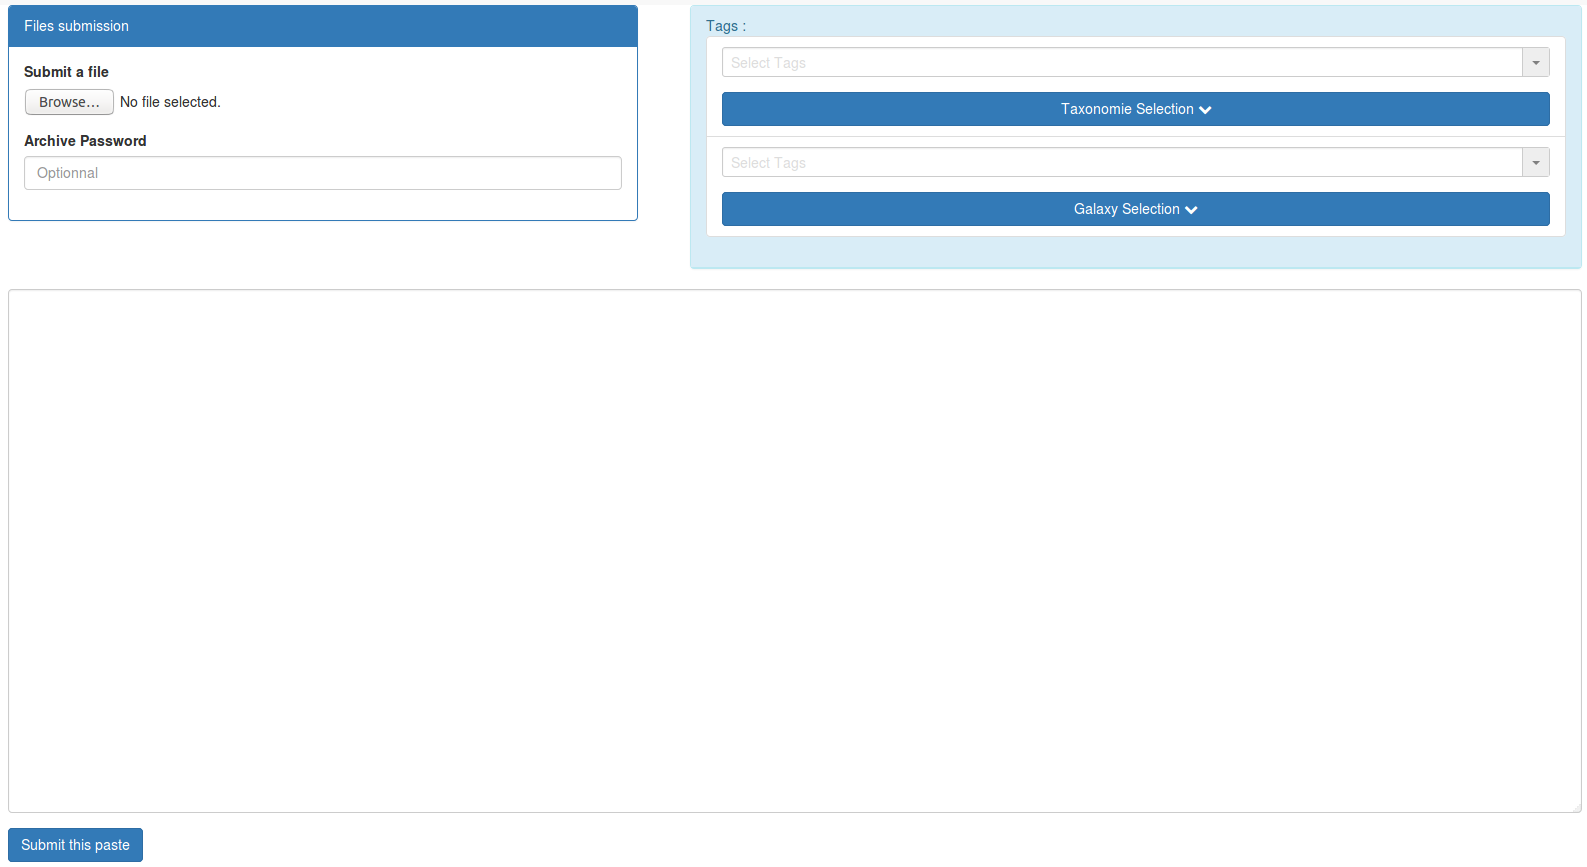
\includegraphics[scale=0.20]{screenshot/paste_submit.png}}
\end{frame}

\begin{frame}
    \frametitle{Via the UI (2)}
    \centerline{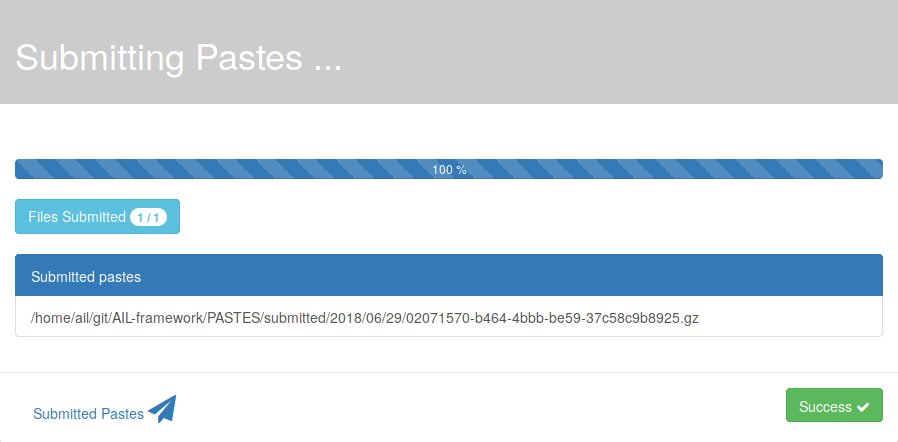
\includegraphics[scale=0.25]{screenshot/paste_submitted.png}}
\end{frame}


%Own data
\begin{frame}
    \frametitle{Feeding AIL with your own data - \texttt{import\_dir.py} (1)}
    /!$\backslash$ One requirement:
    \vskip 1em
    \begin{itemize}
        \item Each file to be fed must be of a raisonable size:
        \begin{enumerate}
            \item \texttt{$\sim$ 3 Mb} is already large
            \item This is because some modules are doing \textbf{regex matching}
            \item If you want to feed a large file, better \textbf{split it in multiple ones}
        \end{enumerate}

    \end{itemize}
\end{frame}

\begin{frame}
    \frametitle{Feeding AIL with your own data - \texttt{import\_dir.py} (2)}
    \begin{enumerate}
        \item Make sure that
            \begin{itemize}
                \item The file \texttt{\large{bin/package/config.cfg}},
                \item Contains the entry \texttt{127.0.0.1:5556} in \texttt{ZMQ\_Global} variable
                \item (It is set by default)
            \end{itemize}
        \pause
        \item Launch \texttt{import\_dir.py} with de directory you want to import
            \begin{itemize}
                \item \texttt{import\_dir.py -d dir\_path}
            \end{itemize}
        \pause
        \item Watch your data being feed to AIL
    \end{enumerate}
\end{frame}

%DEVELOPING NEW FEATURES
\section{Creating new features}
%Modules flow
\begin{frame}
    \frametitle{Developping new features: Plug-in a module in the system}
    \begin{enumerate}
        \item[] Choose where to put your module in the data flow:
    \end{enumerate}
    \begin{figure}
        \centerline{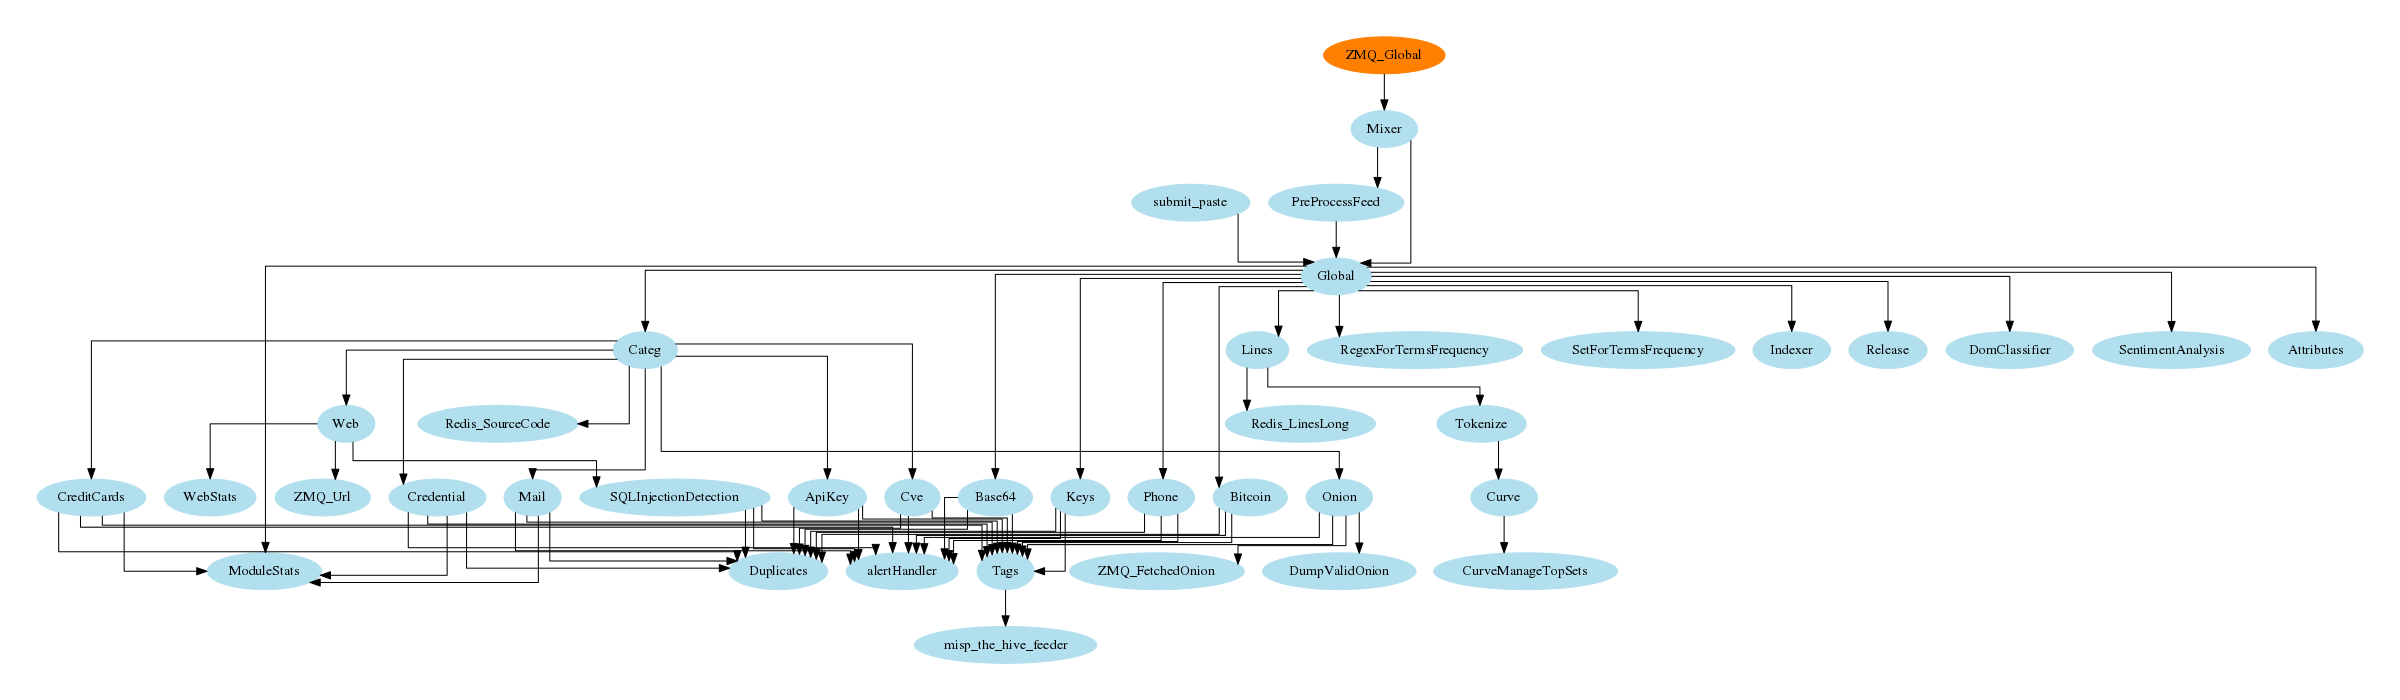
\includegraphics[scale=0.15]{images/module-data-flow.png}}
    \end{figure}
    \vskip -1em
    \begin{enumerate}
        \item[] Then, modify \texttt{bin/package/modules.cfg} accordingly
    \end{enumerate}
\end{frame}


\lstset{style=code}
\lstset{basicstyle=\fontsize{6}{8}\ttfamily}
\begin{frame}[fragile]
    \frametitle{Writing your own modules - \texttt{/bin/template.py}}
    \vspace{-0.5cm}
    \begin{lstlisting}
import time
from pubsublogger import publisher
from Helper import Process
if __name__ == '__main__':
    # Port of the redis instance used by pubsublogger
    publisher.port = 6380
    # Script is the default channel used for the modules.
    publisher.channel = 'Script'
    # Section name in bin/packages/modules.cfg
    config_section = '<section name>'
    # Setup the I/O queues
    p = Process(config_section)
    # Sent to the logging a description of the module
    publisher.info("<description of the module>")
    # Endless loop getting messages from the input queue
    while True:
        # Get one message from the input queue
        message = p.get_from_set()
        if message is None:
            publisher.debug("{} queue is empty, waiting".format(config_section))
            time.sleep(1)
            continue
        # Do something with the message from the queue
        something_has_been_done = do_something(message)
    \end{lstlisting}
\end{frame}

%Flask related
\begin{frame}
    \frametitle{AIL - Add your own web interface}
    \begin{enumerate}
        \item Launch \texttt{var/www/create\_new\_web\_module.py}
        \item Enter the module's name
        \item A template and flask skeleton has been created for your new webpage in \texttt{var/www/modules/}
        \item You can start \textbf{coding} server-side in:
            \begin{itemize}
                \item[] {\scriptsize \texttt{var/www/modules/\textit{your\_module\_name}/Flask\_\textit{your\_module\_name.py}}}
            \end{itemize}
        \item You can start \textbf{coding} client-side in:
            \begin{itemize}
                \item[] {\scriptsize \texttt{var/www/modules/\textit{your\_module\_name}/templates/\textit{your\_module\_name.html}}}
                \item[] {\scriptsize \texttt{var/www/modules/\textit{your\_module\_name}/templates/header\_\textit{your\_module\_name.html}}}
            \end{itemize}
    \end{enumerate}
\end{frame}

\section{Push alert to MISP}
\begin{frame}
    \frametitle{Push alert to MISP}
    \centerline{
        
\includegraphics[scale=0.20]{images/circl-small.png}
        \hskip 2em
        $\longrightarrow$
        \hskip 2em
        
\includegraphics[scale=0.7]{images/MISP.png}
    }

    \vskip 2em
    \textbf{Goal:} push tags to MISP.
\end{frame}

\begin{frame}
    \frametitle{Push alert to MISP}
    \centerline{
        
\includegraphics[scale=0.20]{images/circl-small.png}
        \hskip 2em
        $\longrightarrow$
        \hskip 2em
        
\includegraphics[scale=0.7]{images/MISP.png}
    }

    \vskip 2em
    \begin{enumerate}
            \item Use infoleak taxonomy\footnote{\url{https://www.misp-project.org/taxonomies.html}}
        \item Add your own tags
	\item Create an event on a paste
    \end{enumerate}
\end{frame}

\begin{frame}
    \frametitle{: Finding the best place in the system}
    Best place to put it?
    \centerline{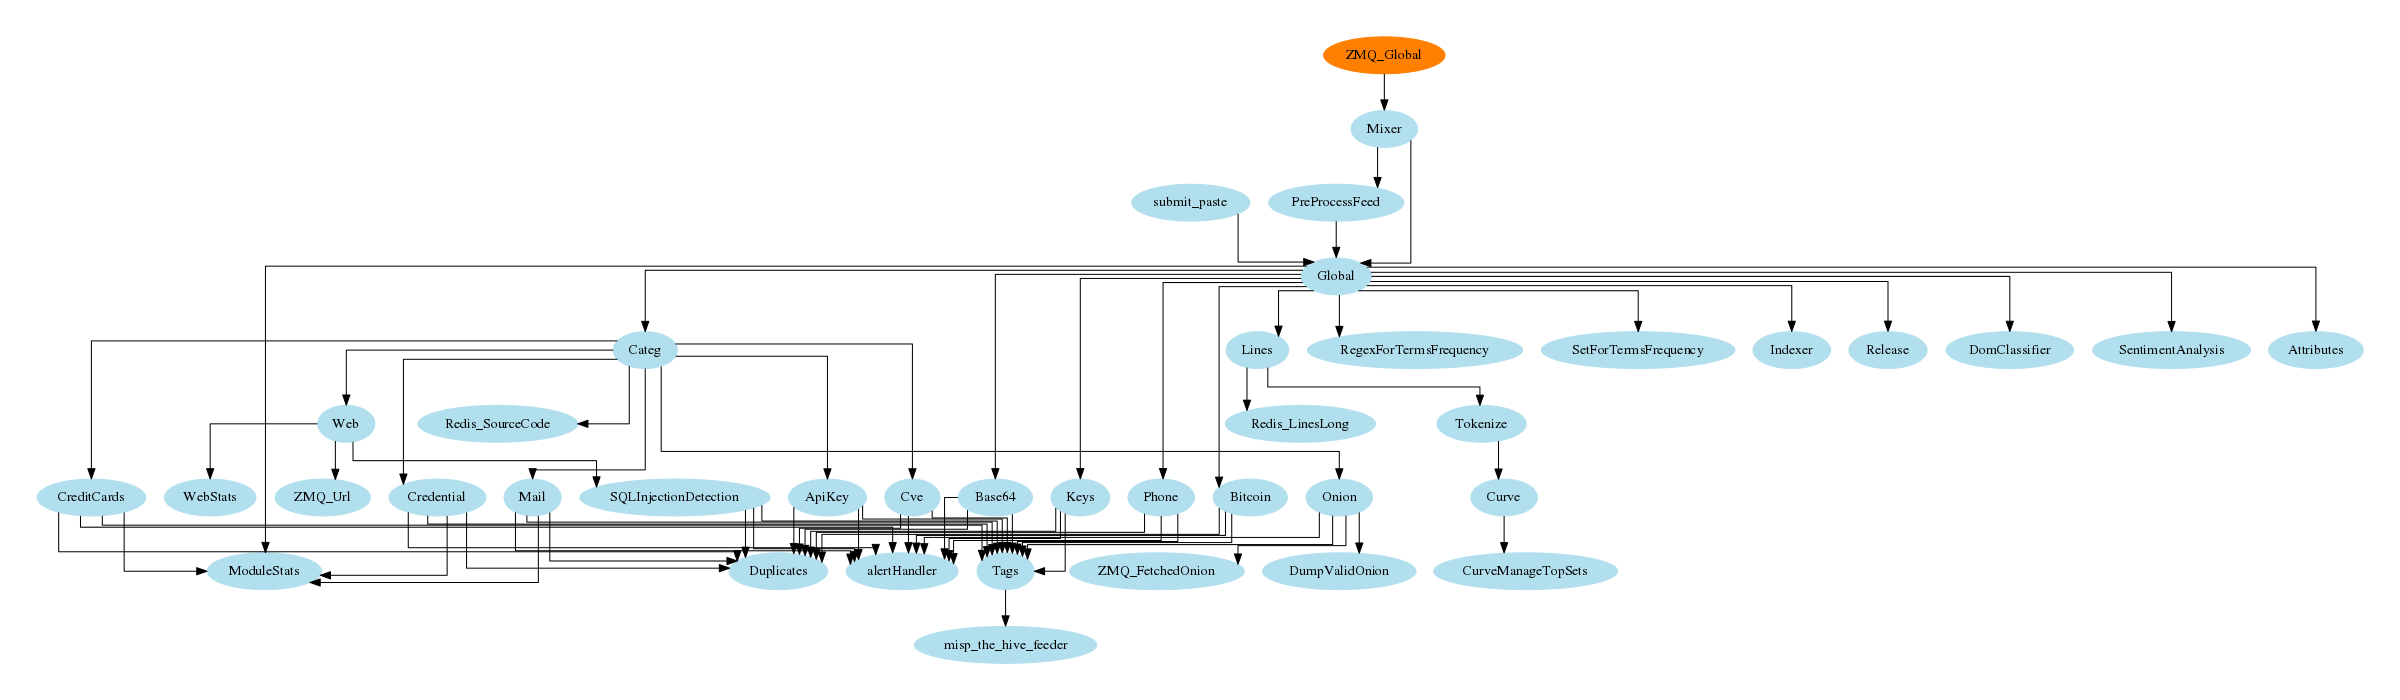
\includegraphics[scale=0.15]{images/module-data-flow.png}}
\end{frame}

\begin{frame}
    \frametitle{: Finding the best place in the system}
    Best place to put it?
    \centerline{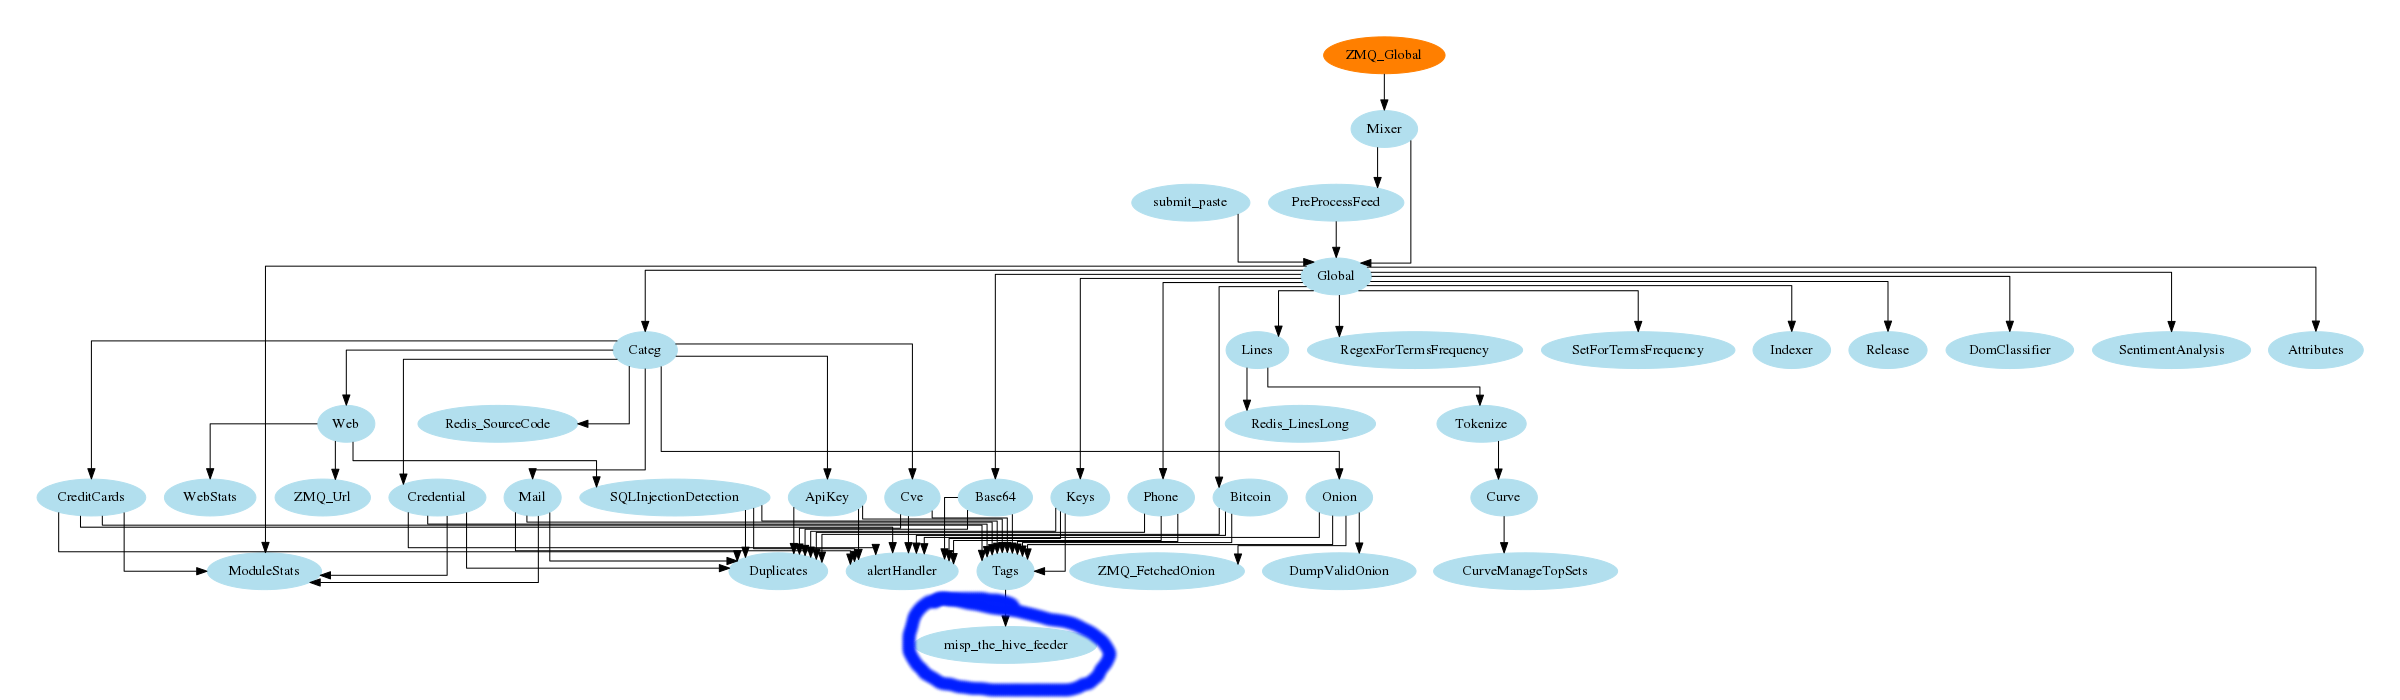
\includegraphics[scale=0.15]{images/module-data-flow-tags-misp-feeder.png}}
\end{frame}

\begin{frame}
    \frametitle{Auto Push Tags}
    \centerline{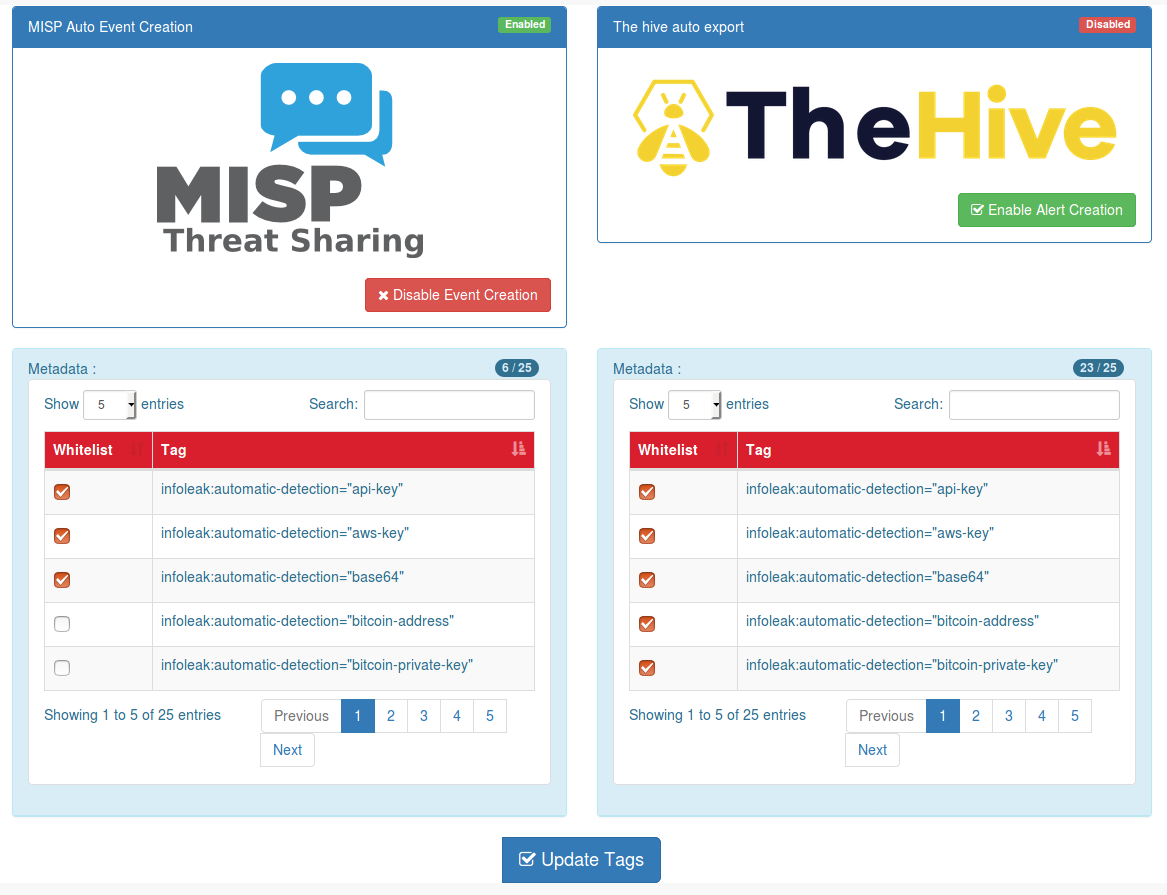
\includegraphics[scale=0.25]{screenshot/tag_auto_export.png}}
\end{frame}

\begin{frame}
    \frametitle{Create an event}
    \centerline{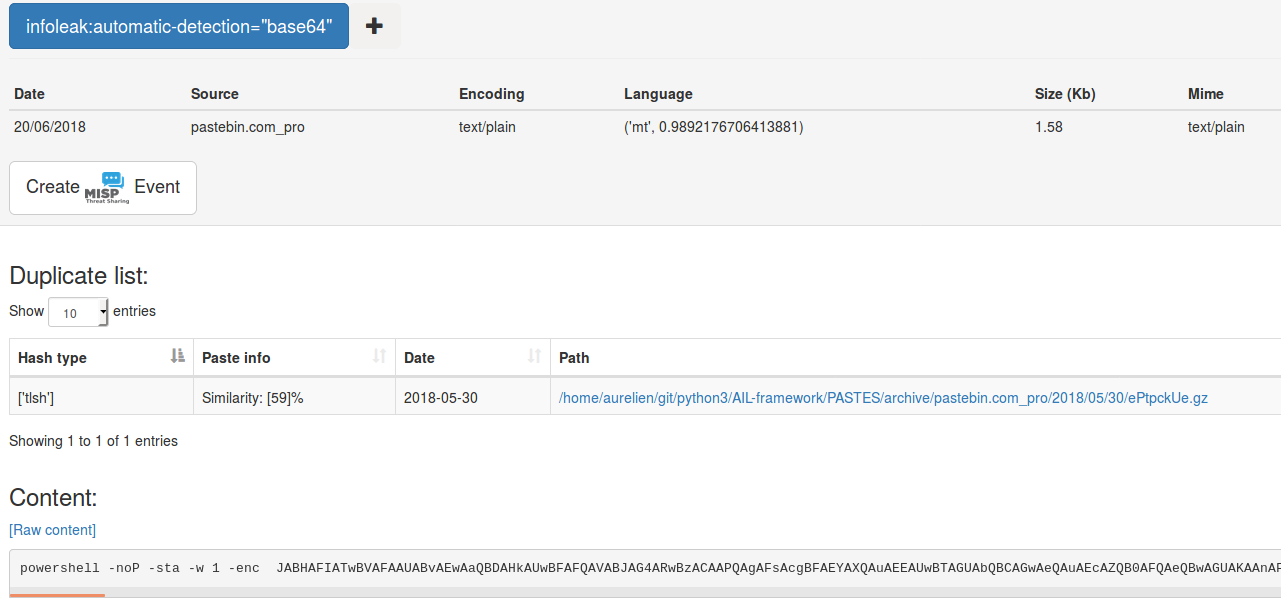
\includegraphics[scale=0.25]{screenshot/create-event-base64.png}}
\end{frame}

\begin{frame}
    \frametitle{Create an event}
    \centerline{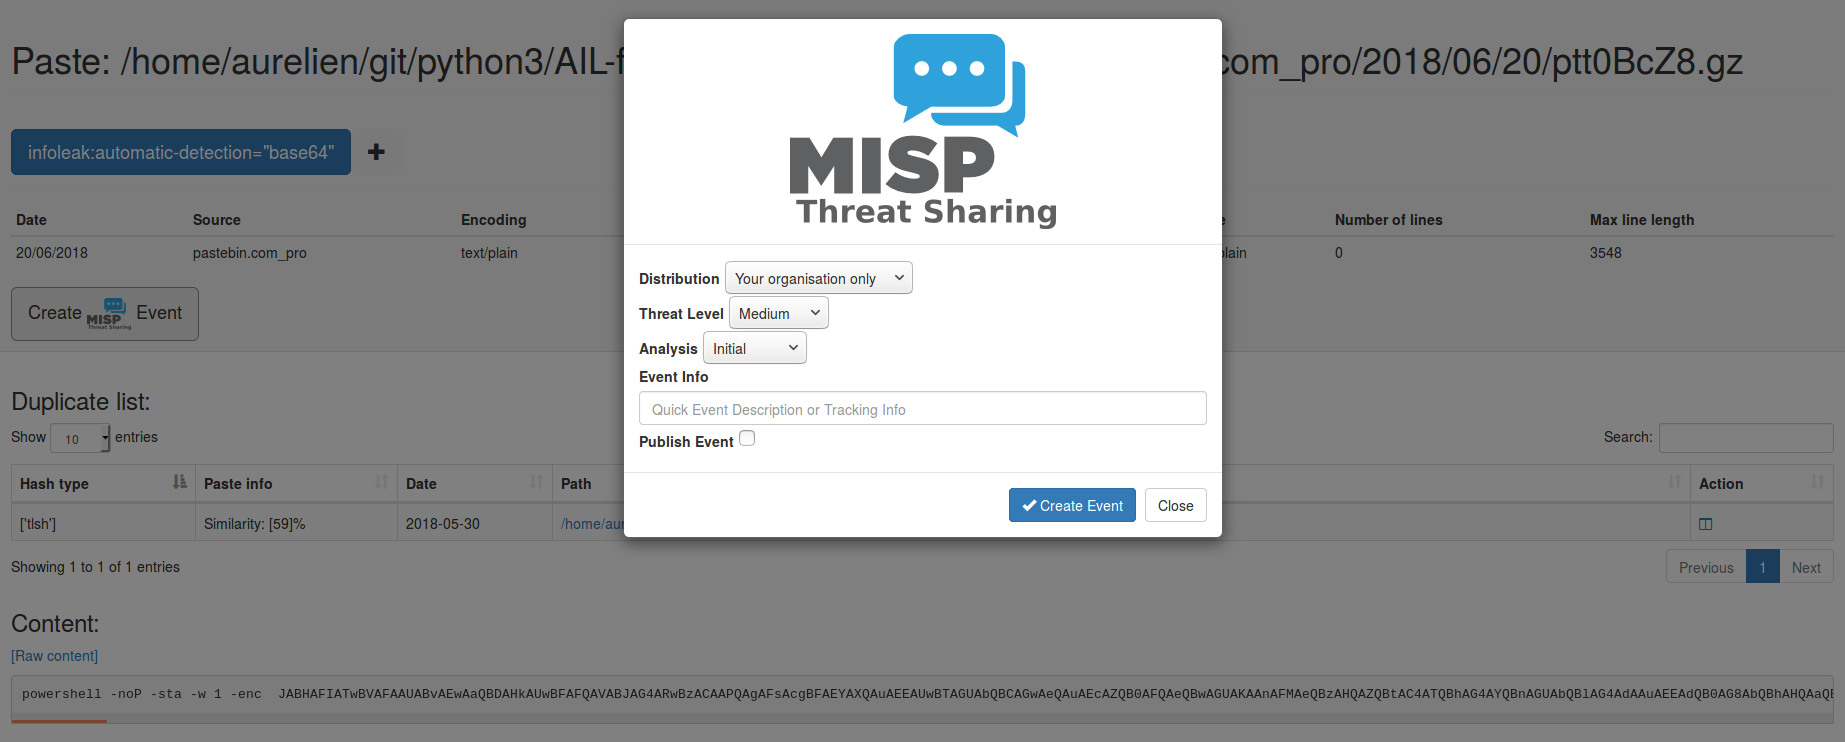
\includegraphics[scale=0.25]{screenshot/create-misp-event-base64.png}}
\end{frame}

\section{Contribution rules}
\begin{frame}
\frametitle{How to contribute}
    \centerline{
\includegraphics[scale=0.5]{images/one-does-not-simply.jpeg}}
\end{frame}

\begin{frame}
    \frametitle{Glimpse of contributed features}
    \begin{itemize}
        \item Docker
        \item Ansible
        \item Email alerting
        \item SQL injection detection
        \item Phone number detection
    \end{itemize}
\end{frame}


\begin{frame}
\frametitle{How to contribute}
%\o/
    \begin{itemize}
        \item Feel free to fork the code, play with it, make some patches or add additional analysis modules.
        \pause
        \item Feel free to make a pull request for your contribution
        \pause
        \item That's it!
    \end{itemize}
    \begin{figure}
        
\includegraphics[scale=0.2]{images/dancing.png}
    \end{figure}
\end{frame}

%%Dashboard empty
%\begin{frame}
%    \frametitle{AIL - Run your own instance}
%    \begin{enumerate}
%        \item[] \url{https://github.com/CIRCL/AIL-framework}
%    \end{enumerate}
%    \begin{figure}
%        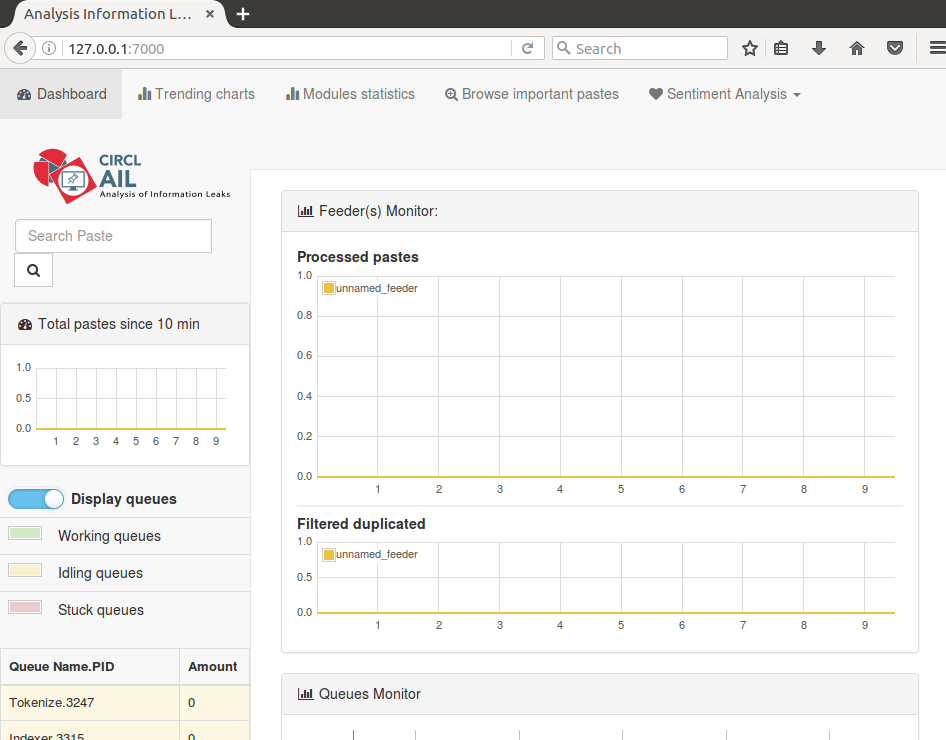
\includegraphics[scale=0.25, angle=0]{images/ail_empty_1min.png}
%    \end{figure}
%\end{frame}
%
%
%%Dashboard pystemon
%\begin{frame}
%    \frametitle{AIL - Run your own instance: With pystemon}
%    \begin{enumerate}
%        \item[] \url{https://github.com/CIRCL/pystemon}
%    \end{enumerate}
%    \begin{figure}
%        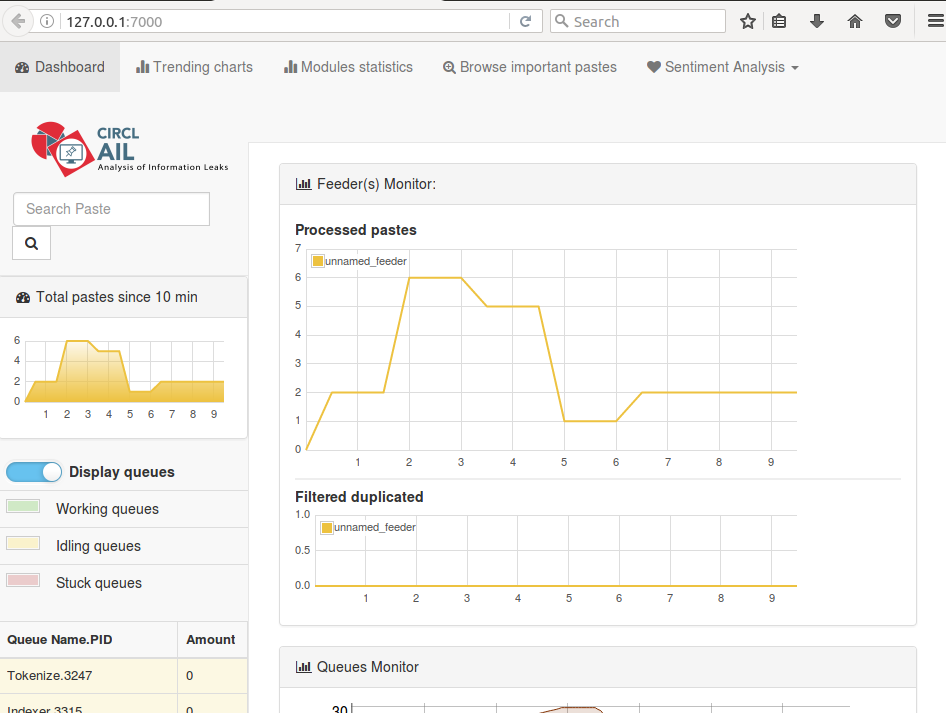
\includegraphics[scale=0.25, angle=0]{images/ail_pyst_10min.png}
%    \end{figure}
%\end{frame}
%
%
%%Dashboard CIRCL feed
%\begin{frame}
%    \frametitle{AIL - Run your own instance: Use CIRCL feed}
%    \begin{enumerate}
%        \item[] Request access at: \href{mailto:info@circl.lu}{info@circl.lu}
%    \end{enumerate}
%    \begin{figure}
%        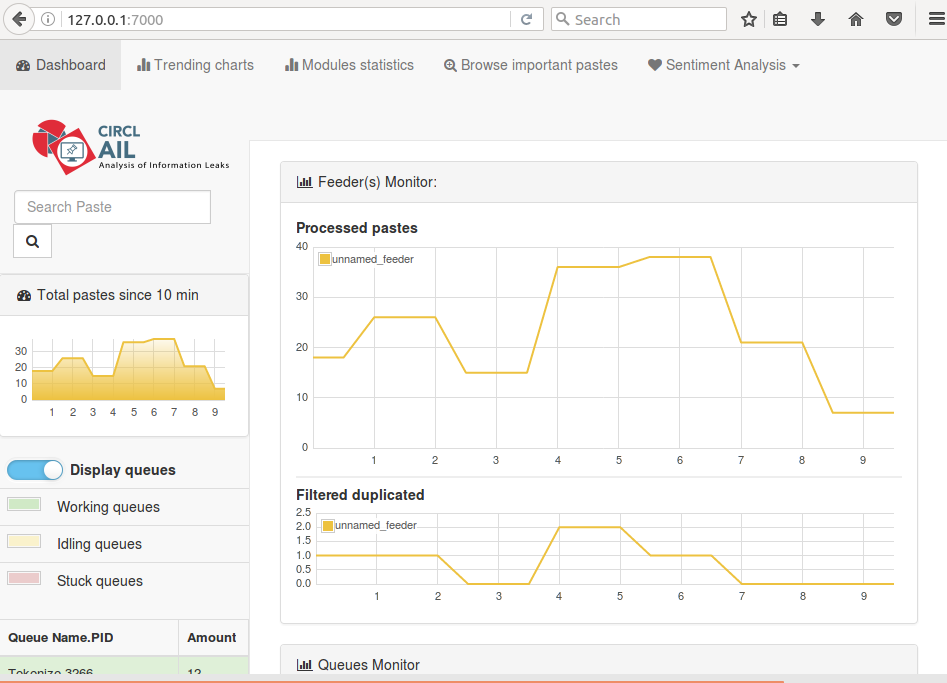
\includegraphics[scale=0.25, angle=0]{images/ail_crf_10min.png}
%    \end{figure}
%\end{frame}

\section{Practical part}
\begin{frame}
    \frametitle{Practical part: Pick your choice}

    \begin{enumerate}
        \item Update support of docker/ansible
        \item Graph database on \texttt{Credential.py}
        \begin{itemize}
            \item Top used passwords, most compromised user, ...
        \end{itemize}
        \item Webpage scrapper
        \begin{itemize}
            \item Download html from URL found in pastes
            \item Re-inject html as paste in AIL
        \end{itemize}
    \item Improvement of \texttt{Phone.py}
        \begin{itemize}
            \item Way to much false positive as of now. Exploring new ways to validate phone numbers could be interesting
        \end{itemize}

        \item \textbf{Your custom feature}
    \end{enumerate}
\end{frame}




\begin{frame}
   \frametitle{Final words}
   \begin{itemize}
        \item Building AIL helped us to find additional leaks which cannot be found using manual analysis and {\bf improve the time to detect duplicate/recycled leaks}.
            \vskip0.5cm
        \item[] $\rightarrow$ Therefore quicker response time to assist and/or inform proactively affected constituents.
   \end{itemize}
\end{frame}


\section{Annexes}
%MANAGING THE SYSTEM
\section{Managing the framework}
\begin{frame}[fragile]
    \frametitle{Managing AIL: Old fashion way}
    \lstset{style=bash}
    \begin{tcblisting}{colback=black!85,coltext=green,listing only,
        title=Access the script screen, fonttitle=\bfseries}
screen -r Script
\end{tcblisting}
\begin{table}
        \caption{GNU screen shortcuts}
    \begin{tabular}{lr}
        \toprule
        Shortcut & Action \\
        \midrule
        C-a d & detach screen \\
        \midrule
        C-a c & Create new window \\
        \midrule
        C-a n & next window screen \\
        \midrule
        C-a p & previous window screen \\
        \bottomrule
    \end{tabular}
\end{table}
\end{frame}


\begin{frame}[fragile]
    \frametitle{Managing your modules: Using the helper}
    \centerline{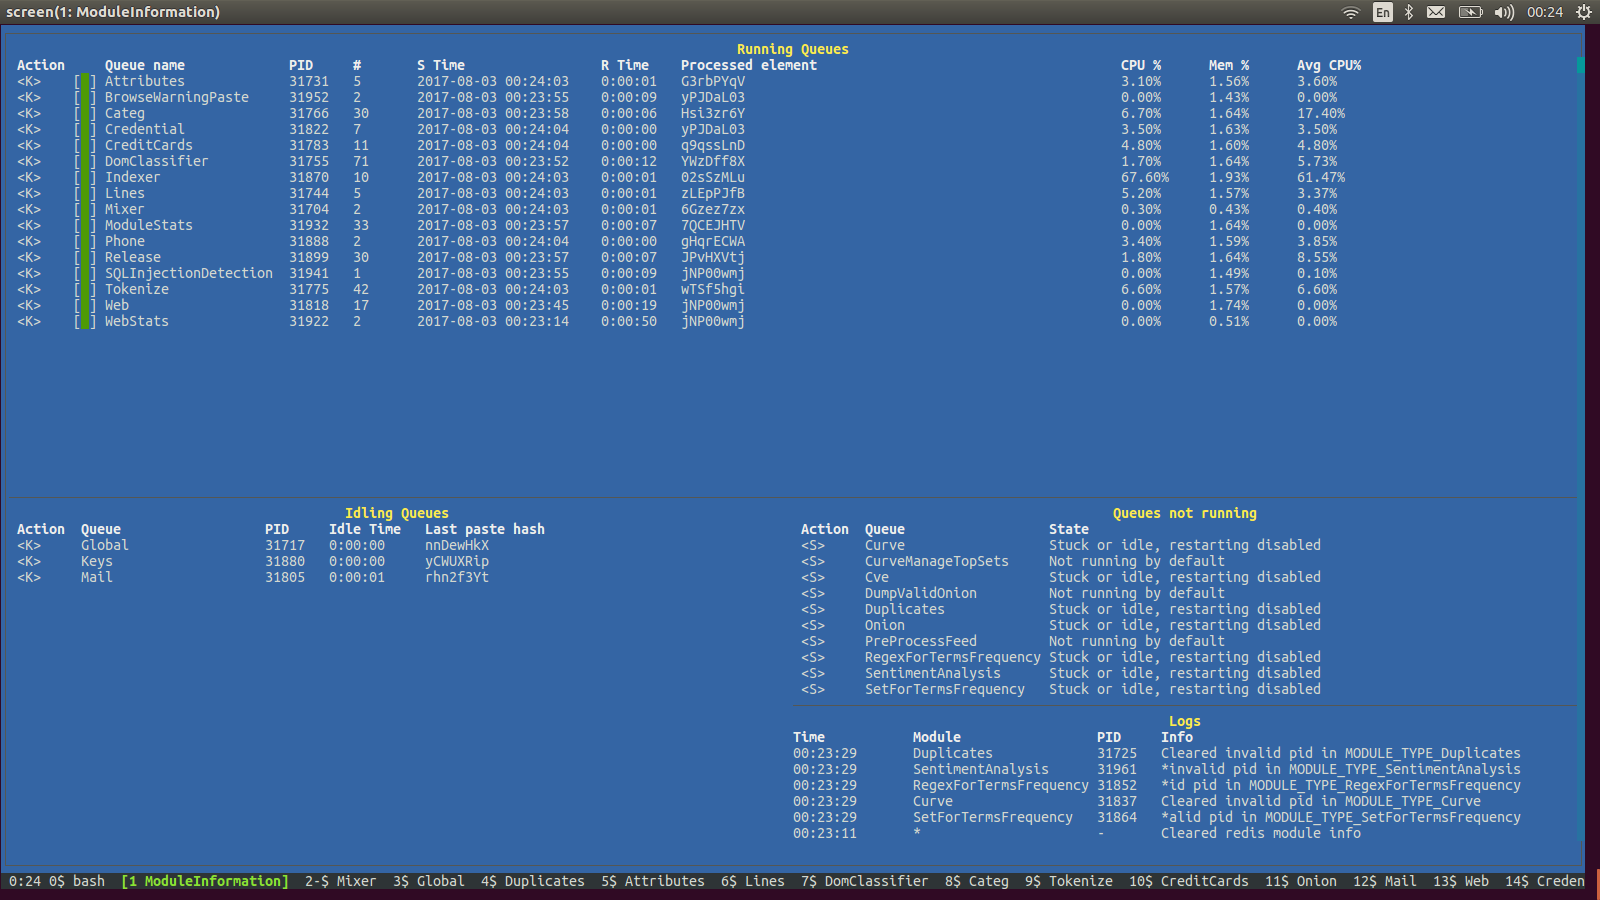
\includegraphics[scale=0.22]{images/moduleManager.png}}
\end{frame}


\end{document}

